%% Control Engineering Practice submission manuscript.
%% Elsevier CAS double-column template, version 2.4 (4 May 2024).
\documentclass[a4paper,fleqn]{cas-dc}
\pdfminorversion=7
\usepackage[numbers,sort&compress]{natbib}
\usepackage{amsmath,amsfonts,amssymb,bm}
\usepackage{mathtools}
\usepackage{xcolor}
\usepackage{algorithmic}
\usepackage{algorithm}
\usepackage{array}
\allowdisplaybreaks
\usepackage{subfig}
\captionsetup[subfloat]{font=small,labelfont=normalfont,
  justification=centering,singlelinecheck=true}
\captionsetup{skip=4pt}
\usepackage{textcomp}
\usepackage{url}
\usepackage{verbatim}
\usepackage{booktabs}
\usepackage{graphicx}
\usepackage{float}
\usepackage{placeins}
\usepackage{multirow}
\usepackage{flushend}
% Permit compact, ordered float packing in the two-column review layout.
\setcounter{topnumber}{4}
\setcounter{bottomnumber}{2}
\setcounter{totalnumber}{6}
\setcounter{dbltopnumber}{2}
\renewcommand{\topfraction}{0.95}
\renewcommand{\bottomfraction}{0.80}
\renewcommand{\textfraction}{0.05}
\renewcommand{\floatpagefraction}{0.88}
\renewcommand{\dbltopfraction}{0.95}
\renewcommand{\dblfloatpagefraction}{0.88}
\setlength{\textfloatsep}{6pt plus 2pt minus 2pt}
\setlength{\floatsep}{5pt plus 2pt minus 2pt}
\setlength{\intextsep}{5pt plus 2pt minus 2pt}
\setlength{\dbltextfloatsep}{6pt plus 2pt minus 2pt}
\setlength{\dblfloatsep}{5pt plus 2pt minus 2pt}
% Elsevier Editorial Manager does not preserve source subdirectories, so the
% submission artwork is kept beside this file in CEP/.
\graphicspath{{./}}
\hyphenation{au-ton-o-mous over-taking race-car}
% Ignore only sub-2-pt class-rounding noise; substantive boxes are fixed below.
\hfuzz=1.95pt
\emergencystretch=2em
\AtBeginDocument{\setlength{\mathindent}{0pt}}

% --- Math shortcuts ---
\newcommand{\R}{\mathbb{R}}
\newcommand{\E}{\mathbb{E}}
\newcommand{\norm}[1]{\left\lVert#1\right\rVert}
\newcommand{\diag}{\operatorname{diag}}
\DeclareMathOperator*{\argmin}{arg\,min}
\DeclareMathOperator*{\argmax}{arg\,max}
\newcommand{\IEEEPARstart}[2]{#1#2}
\newcommand{\IEEEmembership}[1]{#1}

\begin{document}
\let\WriteBookmarks\relax
\def\floatpagepagefraction{1}
\def\textpagefraction{.001}

\shorttitle{Game-Guided Tactical Corridor Learning}
\shortauthors{S. Gao et~al.}

\title[mode=title]{Game-Guided Tactical Corridor Learning for Autonomous Racing Overtakes}

\author[1]{Shuyi Gao}
\author[1]{Ren Jin}
\author[1]{Defu Lin}
% AUTHOR_INPUT_NEEDED: designate the corresponding author and add \ead{...}.

\affiliation[1]{organization={School of Aerospace Engineering, Beijing Institute of Technology},
                  city={Beijing},
                  country={China}}

\begin{abstract}
Interactive overtaking in autonomous racing requires opponent-aware tactical
decisions that remain coherent across repeated replanning and provide a
realizable channel for downstream optimization. We address this
decision-to-execution problem through game-guided tactical-corridor learning.
A robust Stackelberg response-set teacher evaluates near-best opponent
responses and supplies action and value supervision to Truncated Quantile
Critics. The policy publishes a passing-side intention, time-varying Frenet
bounds, and a speed cap. A hysteretic state machine and footprint carver
maintain a connected, side-consistent corridor, which a sequential SOCP, speed
profiler, and nonlinear MPC realize as closed-loop path--speed motion.
Experimental results indicate that the method achieves a 94.7\% overtaking
success rate and a mean overtaking time of 4.82~s. Success exceeded four matched baselines by
31.2--66.2 percentage points; fixed-corridor and no-FSM ablations reduced
success by 18.6 and 12.4 points. These results show that a persistent tactical
feasible region provides an effective interface between interactive decisions
and closed-loop vehicle execution.

\end{abstract}

\begin{keywords}
Autonomous racing \sep game-guided reinforcement learning \sep tactical corridor
\sep interactive overtaking
\end{keywords}

\maketitle

% =====================================================================
\section{Introduction}
% =====================================================================
Autonomous racing combines high speed, narrow maneuvering space, and direct
competition with non-cooperative opponents. During an overtake, relative
geometry and opponent behavior evolve while the planning loop repeatedly
updates its solution. A useful tactical decision must therefore remain
coherent long enough to form a continuous passing channel and must expose that
channel in a form that the path and speed planners can realize. Full-scale
events such as the Abu Dhabi Autonomous Racing League (A2RL) make this
requirement practically important because racing software observes competing
vehicles and returns drive-by-wire commands under a hard real-time loop
~\cite{betz2022survey,hoffmann2026a2rl}. The central problem considered here is
the persistence and executability of opponent-aware overtaking decisions under
repeated replanning.

\subsection{Related work}

Traditional overtaking methods organize interaction through hierarchical
maneuver planning or explicit dynamic games. In hierarchical architectures, a
tactical layer selects among following, defending, and passing behaviors, and a
lower layer converts the selected behavior into a path and speed profile.
Finite-state and candidate-trajectory planners make this decomposition
computationally predictable and allow racing rules, collision checks, and
vehicle constraints to be handled by separate modules
~\cite{sureshbabu2022autopass,kim2023hierarchical}. Full-scale head-to-head
systems retain this modular structure because opponent prediction and local
planning must be updated within tight real-time budgets
~\cite{jung2023iac,hoffmann2026a2rl}. Thakkar et al. formulated the high-level
problem as a discrete racing game that generates target waypoints for either a
multi-agent reinforcement-learning controller or a linear-quadratic Nash-game
controller~\cite{thakkar2024hierarchical}. More recently, Toschi et al.
constructed opponent-aware drivable tunnels, selected a tunnel according to
the current interaction, and optimized a trajectory within it
~\cite{toschi2025modular}. These approaches provide interpretable tactical
logic and a practical path to real-time implementation. Their passing
continuity, however, is principally determined by prescribed state
transitions, candidate selection, or tunnel-selection logic; the strategic
decision itself is not learned as a persistent feasible set that is maintained
across successive planning updates.

Explicit game-theoretic planners model the coupling between competitors more
directly. Non-cooperative dynamic games jointly evaluate progress, collision
avoidance, blocking, and overtaking, producing behaviors such as shielding,
faking, and opportunistic passing that are difficult to obtain from independent
trajectory optimization~\cite{liniger2019game,wang2021game}. Iterative
linear-quadratic approximations reduce the cost of solving nonlinear
multi-player games, but their online burden and local solution quality remain
tied to the interaction model and initialization
~\cite{fridovich2020ilqgames}. Hierarchical Stackelberg formulations separate
the leader's maneuver choice from the follower's response, while payoff
learning adapts the interaction objective from observed behavior
~\cite{ji2023hierarchicalgame,lopez2022payoff}. Level-$K$ reasoning offers a
bounded model of opponent rationality; trajectory mixing can further hedge
against changes in the inferred reasoning level~\cite{ji2024competition}.
Constrained-potential and near-potential formulations instead exploit common
structure in the players' objectives to reduce the online game-solving burden
~\cite{jia2023bayesian,kalaria2025alpha}. Related game formulations have also
been used to balance competing human and automation objectives in robust shared
control~\cite{swain2023cooperative}. Collectively, these methods make strategic
coupling explicit, yet most publish a maneuver, waypoint sequence, or selected
trajectory at each update. Consequently, side commitment and the spatial
freedom available to the downstream planner must still be reconstructed by an
additional temporal logic layer.

Learning-based methods replace repeated online search with a fixed-cost policy
evaluation and can acquire interaction patterns directly from competitive
experience. Curriculum learning has produced overtaking policies by gradually
increasing opponent difficulty, while large-scale deep reinforcement learning
has demonstrated high-performance racing and human-like tactical behavior in
simulation~\cite{song2021overtaking,fuchs2021superhuman,wurman2022gtsophy}.
Comparisons with optimal control show that reinforcement learning can exploit
complex racing dynamics effectively, although its behavior depends strongly on
the training distribution and reward design~\cite{lin2023limit}. To introduce
more structure, trajectory-aided policies condition learning on a nominal path,
LiDAR-based agents learn directly from local perception, and predictive
planners incorporate an opponent forecast into overtaking-trajectory
generation~\cite{evans2023trajectory,hell2024lidar,
baumann2025predictive}. Game-informed deep reinforcement learning couples the
policy reward to another vehicle's action, whereas dynamic-graph and
multi-agent formulations encode pairwise relations or coordinated behavior
among several vehicles~\cite{yuan2022drlgame,hu2023dynamicgraph,
han2024marl}. These designs improve interaction awareness, but an end-to-end
control action or a single learned trajectory offers little freedom for a
constrained planner to reshape the maneuver when the opponent moves during the
pass.

Hybrid learning--optimization architectures therefore expose an intermediate
decision to a model-based planner. Reiter et al. used reinforcement learning to
parameterize the objective of a nonlinear predictive planner, confining
exploration to trajectories accepted by the optimizer
~\cite{reiter2023hierarchical}. In road-traffic applications, learned tactical
layers have been used to anticipate disruptive lane changes and to coordinate
merging sequences subsequently realized by optimal control
~\cite{liu2023proactive,muzahid2025merging}. Human feedback provides another
source of policy guidance for stabilizing learned driving strategies
~\cite{guo2025rlhf}. Most closely related to a corridor interface, Yang et al.
used MARL-generated cooperative reference trajectories to construct
spatio-temporal corridors for downstream optimization
~\cite{yang2026corridor}, while Toschi et al. computed alternative drivable
tunnels from predicted track occupancy~\cite{toschi2025modular}. The present
problem differs in the interaction model and in what is learned: the vehicles
are non-cooperative, and the policy directly publishes a side-locked feasible
region rather than a guiding trajectory or a selector over independently
generated tunnels.

The literature thus provides effective game models, learned tactical policies,
and corridor-constrained planners, but leaves a specific coupling problem
between them. During a close overtake, opponent-aware reasoning must remain
consistent across policy updates while preserving sufficient geometric freedom
for receding-horizon planning. We address this problem by representing the
decision as a persistent tactical feasible region. A robust Stackelberg
response-set teacher evaluates projected candidates against near-best opponent
responses, TQC distils the resulting action and value supervision into one
policy evaluation, and deterministic hybrid logic maintains the selected side
while publishing time-varying Frenet bounds and a speed request. This design
transfers strategic interaction reasoning to the planner without reducing the
decision to a single path.

\subsection{Contributions and paper organization}

This paper formulates interactive overtaking as persistent tactical
feasible-set generation. The proposed policy learns where and when to commit,
preserves the selected side as the encounter evolves, and communicates the
decision to the planner through explicit space--speed bounds. A common
model-based executor then realizes these bounds as a continuous path--speed
reference and closed-loop vehicle motion.

The contributions are threefold.
\begin{enumerate}
    \item We construct a robust Stackelberg response-set teacher that evaluates
    projected tactical candidates against near-best opponent responses. Its
    response-set-optimal action prior and action-conditioned value labels guide
    TQC toward overtaking opportunities that retain progress and clearance
    across plausible interaction outcomes.

    \item We introduce a planner-compatible tactical representation that
    combines a learned time-varying corridor with hysteretic side commitment,
    deterministic opponent-footprint carving, and reference-level
    tire-admissibility projection. The resulting interface maintains a
    connected passing region and consistent side choice while the relative
    geometry changes.

    \item We evaluate decision persistence and planner executability in a
    target-hardware HIL loop. Matched baselines and ablations isolate how
    corridor shaping, side commitment, game supervision, and distributional
    learning affect overtaking success and closed-loop feasibility.
\end{enumerate}

Section~\ref{sec:model} formulates the overtaking problem and vehicle--track
models. Section~\ref{sec:tactical} presents the game-guided corridor policy.
Section~\ref{sec:execution} summarizes the common corridor-constrained
reference-generation and closed-loop tracking layer. Section~\ref{sec:experiments} reports the HIL evaluation, comparative
analysis, and validation scope.

% =====================================================================
\begingroup
\setlength{\abovedisplayskip}{6pt plus 1pt minus 1pt}
\setlength{\belowdisplayskip}{6pt plus 1pt minus 1pt}
\setlength{\abovedisplayshortskip}{4pt plus 1pt minus 1pt}
\setlength{\belowdisplayshortskip}{4pt plus 1pt minus 1pt}
\setlength{\jot}{2pt}
\section{Problem description and modeling}
\label{sec:model}
% =====================================================================
Figure~\ref{fig:vehicle_track_model} shows the two-vehicle overtaking scenario
considered in this study. An ego race car must pass a non-cooperative opponent
on a closed track by selecting a persistent passing side, Frenet corridor, and
speed request from the vehicle states and local track geometry. The following
models define the vehicle and interaction quantities used by the tactical
policy and executor.

For vehicle $i\in\{e,o\}$, $(X_i,Y_i,\psi_i)$ denotes the inertial
pose and $(v_{x,i},v_{y,i},r_i)$ the body-frame velocity and yaw rate, with
$V_i=\sqrt{v_{x,i}^2+v_{y,i}^2}$ and
$\beta_i=\operatorname{atan2}(v_{y,i},v_{x,i})$. Let
$\mathcal W=\{\mathrm{fl},\mathrm{fr},\mathrm{rl},\mathrm{rr}\}$, and let
$\bm r_q=[x_q,y_q]^\top$ and $\delta_q$ denote the position and steering
angle of wheel $q$. The front wheels share the commanded steering angle and
the rear wheels are unsteered. The planar four-wheel dynamics are
\begin{equation}
\begin{bmatrix}
\dot X_i\\
\dot Y_i\\
\dot\psi_i\\
\dot v_{x,i}\\
\dot v_{y,i}\\
\dot r_i
\end{bmatrix}
=
\begin{bmatrix}
v_{x,i}\cos\psi_i-v_{y,i}\sin\psi_i\\
v_{x,i}\sin\psi_i+v_{y,i}\cos\psi_i\\
r_i\\
\begin{gathered}
\displaystyle\frac{1}{m}\sum_{q\in\mathcal W}
(F_{x,q}\cos\delta_q-F_{y,q}\sin\delta_q)+r_iv_{y,i}\\[-1mm]
\displaystyle{}-\frac{F_{\rm drag}(V_i)}{m}
\end{gathered}\\[3mm]
\displaystyle\frac{1}{m}\sum_{q\in\mathcal W}
(F_{x,q}\sin\delta_q+F_{y,q}\cos\delta_q)-r_iv_{x,i}\\[3mm]
\begin{gathered}
\displaystyle\frac{1}{I_z}\sum_{q\in\mathcal W}
\bigl[x_q(F_{x,q}\sin\delta_q+F_{y,q}\cos\delta_q)\\[-1mm]
\displaystyle{}-y_q(F_{x,q}\cos\delta_q-F_{y,q}\sin\delta_q)\bigr]
\end{gathered}
\end{bmatrix}.
\label{eq:vehicle_dynamics}
\end{equation}
where $m$ and $I_z$ are the vehicle mass and yaw inertia, and
$F_{\rm drag}$ is the aerodynamic drag force. Pure-slip tire forces and the
resulting quasi-steady-state acceleration envelope are described by
\begin{equation}
\begin{aligned}
\zeta_{d,q}&=B_d\chi_{d,q}-E_d\bigl(B_d\chi_{d,q}
-\arctan(B_d\chi_{d,q})\bigr),\\
F_{d,q}(\chi_{d,q},F_{z,q})
&=D_d(F_{z,q})\sin\!\bigl(C_d\arctan\zeta_{d,q}\bigr),\\
D_d(F_{z,q})&=F_{z,q}\!\left[\mu_d+s_d
\frac{F_{z,q}-F_{z,0}}{F_{z,0}}\right],\\
B_d&=\frac{\tan\!\left(\pi/(2C_d)\right)}{q_{d,\rm pk}},
\qquad d\in\{x,y\},\ q\in\mathcal W,\\
\begin{bmatrix}a_T\\a_N\end{bmatrix}
&=\frac{1}{m}\sum_{q\in\mathcal W}
\bm R(\delta_q-\beta_i)
\begin{bmatrix}F_{x,q}\\F_{y,q}\end{bmatrix},\\
\bm R(\varphi)&=
\begin{bmatrix}\cos\varphi&-\sin\varphi\\
\sin\varphi&\cos\varphi\end{bmatrix},\\
\mathcal A_{\rm tire}(V)
&=\{(a_T,a_N):\Phi_{\rm tire}(a_T,a_N,V)\le1\}.
\end{aligned}
\label{eq:tire_accel_envelope}
\end{equation}
Here $\chi_{x,q}=\lambda_q$, $\chi_{y,q}=\alpha_q$, and $E_d=0$ for the
fitted curves. Following \cite{veneri2020free}, the envelope is stored as a
speed-interpolated map whose traction and braking limits are
$a_{T,{\rm env}}^{+}(a_N,V)$ and $b_{T,{\rm env}}^{-}(a_N,V)$.

Let $\bm r_c(s)$ denote the track centerline parameterized by arc length
$s\in[0,L_{\rm trk})$, with tangent angle $\theta(s)$ and curvature
$\kappa(s)=d\theta/ds$. The Frenet geometry and kinematics are
\begin{equation}
\begin{aligned}
\bm t(s)&=[\cos\theta(s),\sin\theta(s)]^\top,\\
\bm n_c(s)&=[-\sin\theta(s),\cos\theta(s)]^\top,\\
\bm p_i&=[X_i,Y_i]^\top=\bm r_c(s_i)+n_i\bm n_c(s_i),\quad
\xi_i=\psi_i-\theta(s_i),\\
v_{s,i}&=V_i\cos(\xi_i+\beta_i),\qquad
v_{n,i}=V_i\sin(\xi_i+\beta_i),\\
\begin{bmatrix}\dot s_i\\\dot n_i\\\dot\xi_i\end{bmatrix}
&=
\begin{bmatrix}
v_{s,i}/(1-\kappa(s_i)n_i)\\
v_{n,i}\\
r_i-\kappa(s_i)v_{s,i}/(1-\kappa(s_i)n_i)
\end{bmatrix}.
\end{aligned}
\label{eq:frenet_kinematics}
\end{equation}
The lateral coordinate is positive to the left, with
$n_{\rm trk}^{-}(s)\le n\le n_{\rm trk}^{+}(s)$. The spatial model is used
within $1-\kappa n\ge\varepsilon_s$, $|\xi|\le\xi_{\max}<\pi/2$, and
$v_s\ge\underline v_s>0$; Table~\ref{tab:setup_params} lists the limits.

\begin{figure}[t]
\centering
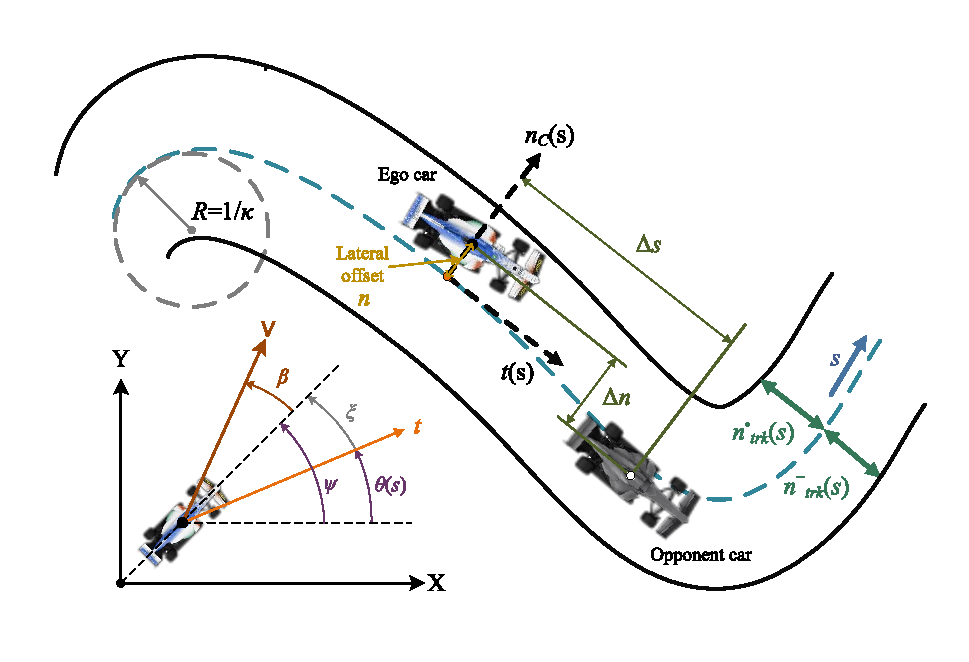
\includegraphics[width=\linewidth]{model_shuoming_corrected.pdf}
\caption{Vehicle motion and relative geometry in the Frenet frame.}
\label{fig:vehicle_track_model}
\end{figure}

Centerline projection, unwrapped at the start--finish line, gives the relative
ego--opponent quantities
\begin{equation}
\begin{aligned}
g=\Delta s
&=\bigl((s_o-s_e+L_{\rm trk}/2)\bmod L_{\rm trk}\bigr)-L_{\rm trk}/2,\\
\Delta n&=n_o-n_e,\qquad \Delta v=v_{s,e}-v_{s,o}.
\end{aligned}
\label{eq:rel}
\end{equation}
Here $g>0$ denotes an opponent ahead and $\Delta v>0$ denotes the ego closing;
these variables describe the duel geometry used by the tactical policy.

For spatial path generation, $s$ is the independent variable,
$\bm z(s)=[n(s),\xi(s)]^\top$ is the geometric state, and $\omega(s)$ is the
path curvature. The resulting model is
\begin{equation}
\bm z'(s)=\bm f_s(\bm z,\omega;s)=
\begin{bmatrix}
(1-\kappa n)\tan\xi\\[2pt]
(1-\kappa n)\omega/\cos\xi-\kappa
\end{bmatrix}.
\label{eq:spatial_model}
\end{equation}
Section~\ref{sec:planner} uses its first-order approximation in the sequential
SOCP.

% Condensed Sections 3--4: the tactical contribution is kept explicit, while
% standard execution details are summarized to preserve experimental space.

% =====================================================================
\section{Game-Guided Tactical Corridor Policy}\label{sec:tactical}
% =====================================================================
The tactical layer converts opponent-aware interaction reasoning into a
persistent feasible region. Response-set supervision identifies overtaking
opportunities across plausible opponent reactions, TQC amortizes this
reasoning into a real-time policy, and the hybrid publisher maintains the
selected side while constructing explicit corridor bounds for the planner.

\subsection{Robust Stackelberg response-set supervision}
\label{subsec:game_formulation}
At each tactical update, the encoder combines the two vehicle states, local
track preview, current mode, side lock, and execution health into
$\widetilde{\bm o}_t$. The actor produces
\begin{equation}
\begin{aligned}
\bm a^{\rm raw}=\bigl[&L^{\rm cap},R^{\rm cap},d_{\rm safe},
V_{\rm cap}^{\rm req},g_{\rm chase},\\[-1mm]
&g_{\rm ot},g_{\rm abort},b_{\rm lat},w_{\rm safe},
q_{\rm side}\bigr]^\top .
\end{aligned}
\label{eq:action_vec}
\end{equation}
where the components specify the usable track widths, footprint margin,
requested speed cap, ordered interaction distances, defensive interval, and
side intention. Together, these variables describe the spatial extent,
timing, and side commitment of the passing opportunity. The Euclidean
projection $\Pi_{\mathcal A}$ enforces the component bounds in
Table~\ref{tab:tactical_settings}, the guard order
$g_{\rm ot}+\Delta_g\le g_{\rm chase}\le g_{\rm abort}-\Delta_g$, and the
minimum corridor width. The tactical action therefore follows the single
chain
\[
\bm a^{\rm raw}\xrightarrow{\Pi_{\mathcal A}}\bm a^{\rm B}
\xrightarrow{\Pi_{\rm tire}}\bm a^{\rm F},\qquad
\mathcal G_t=(m_{t+1},\sigma_{t+1}^{\rm lock},
V_{{\rm cap},t}^{\rm F},\mathcal C_t).
\]
The neural policy determines the tactical sample; mode, lock, corridor, and
speed-cap publication are resolved by Algorithm~\ref{alg:tactical_corridor}.

The offline teacher forms deterministic leader and follower banks by combining
the three side codes with a Sobol design over the remaining action components.
Every candidate is passed through the same bound projection, corridor carver,
and tire screen used online; duplicate or infeasible candidates are discarded.
Let
\(
\bm s_t^G=(\widetilde{\bm o}_t,\bm\chi_t^G)
\)
denote the teacher state, where $\bm\chi_t^G$ collects the publisher,
executor, and one-step reward memory carried between tactical updates, and
let $\mathcal A_i^G(\bm s_t^G)$ denote the candidate bank for role $i$.
Each candidate pair induces the coupled executable preview
\begin{equation}
(\mathcal R_e,\mathcal R_o)=
\mathscr P_{N_{\rm sta}}\!\left(
\bm s_t^G;\bm a_e^{\rm F},\bm a_o^{\rm F}\right),
\label{eq:coupled_game_preview}
\end{equation}
where $\mathscr P_{N_{\rm sta}}$ recursively applies the stateful publisher
in Algorithm~\ref{alg:tactical_corridor} and the common execution stack.
The candidate pair remains fixed over the preview while both vehicle and
hybrid states evolve jointly; both utilities use the corresponding
role-relative features of this preview.

Let
\(
Z_g=\sum_{k=0}^{N_{\rm sta}-1}\gamma_g^k
\)
and
\(
c_w=\sum_{j=1}^{10}[-w_j]_+
\).
The normalized role-relative utility is
\begin{equation}
\begin{aligned}
U_i(\bm s_t^G,\bm a_e^{\rm F},\bm a_o^{\rm F})
&=\frac{1}{Z_g\|\bm w\|_1}
\sum_{k=0}^{N_{\rm sta}-1}\gamma_g^k\\[-1mm]
&\quad{}\left[\bm w^\top\bm\phi_{i,k}(\mathcal R_e,\mathcal R_o)+c_w\right],
\end{aligned}
\label{eq:game_utility}
\end{equation}
where $\bm\phi_i\in[0,1]^{10}$ contains the role-relative reward features in
\ref{app:parameters}. Hence $U_i\in[0,1]$, and
$\varepsilon_{\rm BR}$ directly specifies the admissible follower-utility gap.
\begin{equation}
\begin{aligned}
U_o^{\max}(\bm s_t^G,\bm a_e^{\rm F})
&=\max_{\bm a_o^{\rm F}\in\mathcal A_o^G(\bm s_t^G)}
U_o(\bm s_t^G,\bm a_e^{\rm F},\bm a_o^{\rm F}),\\
\mathfrak R_o^\varepsilon(\bm s_t^G,\bm a_e^{\rm F})
&=\left\{\bm a_o^{\rm F}\in\mathcal A_o^G(\bm s_t^G):\right.\\[-1mm]
&\qquad\left.
U_o^{\max}(\bm s_t^G,\bm a_e^{\rm F})
-U_o(\bm s_t^G,\bm a_e^{\rm F},\bm a_o^{\rm F})
\le\varepsilon_{\rm BR}\right\},\\
\mathcal V_g(\bm s_t^G,\bm a_e^{\rm F})
&=\min_{\bm a_o^{\rm F}\in
\mathfrak R_o^\varepsilon(\bm s_t^G,\bm a_e^{\rm F})}
U_e(\bm s_t^G,\bm a_e^{\rm F},\bm a_o^{\rm F}),\\
\bm a_{\rm th}^{\star}(\bm s_t^G)
&\in\argmax_{\bm a_e^{\rm F}\in\mathcal A_e^G(\bm s_t^G)}
\mathcal V_g(\bm s_t^G,\bm a_e^{\rm F}),\\
\mathcal D_g
&=\left\{(\widetilde{\bm o}_n,\bm a_{g,n}^{\rm F},v_{g,n},\right.\\[-1mm]
&\qquad\left.
\bm a_{{\rm th},n}^{\star}):
v_{g,n}=\mathcal V_g(\bm s_n^G,\bm a_{g,n}^{\rm F})\right\}.
\end{aligned}
\label{eq:response_set_teacher}
\end{equation}
Here $\varepsilon_{\rm BR}=0.05$ retains responses within $0.05$ of the best
candidate on the normalized utility scale.

Before publication, the requested speed cap is certified against the
speed-dependent tire envelope on the provisional corridor midpoint. For each
trial $v\in\mathcal V_s(V_{\rm cap}^{\rm req})$, define the envelope-unclipped
kinetic-energy template
\begin{equation}
\lambda_k=
\frac{\sum_{j=0}^{k-1}\Delta\ell_j}
{\sum_{j=0}^{N_{\rm sta}-2}\Delta\ell_j},
\qquad
\widehat V_k(v)=
\sqrt{V_e^2+\lambda_k\bigl(v^2-V_e^2\bigr)}.
\label{eq:tire_speed_template}
\end{equation}
Using the midpoint curvature $\widehat\kappa_k$, the induced demand and total
projection are
\begin{equation}
\begin{aligned}
\widehat a_{T,k}(v)
&=\frac{\widehat V_{k+1}^2(v)-\widehat V_k^2(v)}{2\Delta\ell_k}
+\frac{F_{\rm drag}(\widehat V_k(v))}{m},\\
\widehat a_{N,k}(v)
&=\widehat\kappa_k\widehat V_k^2(v),\\
\widehat\rho(v)
&=\max_{0\le k\le N_{\rm sta}-2}\Phi_{\rm tire}\!\left(
\widehat a_{T,k}(v),\widehat a_{N,k}(v),\widehat V_k(v)\right),\\
\mathcal V_{\rm adm}(\bm a)
&=\left\{v\in\mathcal V_s(V_{\rm cap}^{\rm req}):
\widehat\rho(v)\le1\right\},\\
\Pi_{\rm tire}(\bm a;\widetilde{\bm o})
&=\begin{cases}
\bm a[\max\mathcal V_{\rm adm}(\bm a)],
&\mathcal V_{\rm adm}(\bm a)\neq\varnothing,\\
\bm a_{\rm HF}^{\rm F}(\widetilde{\bm o}),
&\mathcal V_{\rm adm}(\bm a)=\varnothing.
\end{cases}
\end{aligned}
\label{eq:tire_safe_action}
\end{equation}
Here $V_e$ is the current ego speed, $\mathcal V_s$ is the uniformly sampled
finite grid from $V_{\min}$ to $V_{\rm cap}^{\rm req}$, and $\bm a[v]$ changes
only the cap component. The total branch $\bm a_{\rm HF}^{\rm F}$ performs the
current-state \textsc{Hold} reconstruction and returns the braking-fallback
contract if its repeated search remains empty.

\subsection{Game-guided distributional policy}
\label{subsec:theory_guided_rl}
The real-time policy maps the evolving duel geometry to the tactical feasible
set at a fixed computational cost. Its 51-dimensional observation concatenates 27 duel-state features with two
12-dimensional track summaries centred at the ego and opponent. The duel
features contain normalized Frenet states and accelerations, relative progress,
lateral gap and closing rate, time to contact, closing-speed code, side lock, and a
nine-state race-mode code. Each track summary reports mean curvature, peak
absolute curvature, and minimum width over four consecutive bins.

The environment reward is
\begin{equation}
\begin{aligned}
r_t&=\bm w^\top\bm\phi_t,\\
\bm\phi_t&=[\phi_{\rm ot},\phi_{\rm ovb},\phi_{\rm col},\phi_{\rm lat},
\phi_{\rm crush},\phi_{\rm app},\\[-1mm]
&\hspace{9mm}\phi_{\rm sm},\phi_{\rm gs},\phi_{\rm sbs},
\phi_{\rm wide}]^\top .
\end{aligned}
\label{eq:reward_sum}
\end{equation}
\ref{app:parameters} gives the normalized definitions and weights.
The same role-swapped features define Eq.~\eqref{eq:game_utility}, aligning the
teacher and online reward at the level of overtaking progress, clearance,
smoothness, and usable corridor width.

\emph{Projected-action TQC.} Truncated Quantile Critics
(TQC)~\cite{kuznetsov2020tqc} discard the largest
target atoms before the quantile-Huber backup. Environment replay $\mathcal D$
stores the final tactical action $\bm a_t^{\rm F}$. For a raw target-policy
sample, the projected action and truncated target are
\begin{equation}
\begin{aligned}
\bm a_{t+1}^{\rm F}&=\Pi_{\rm tire}\!\left(
\Pi_{\mathcal A}(\bm a_{t+1}^{\rm raw});
\widetilde{\bm o}_{t+1}\right),\\
\ell_{t+1}&=\log\pi_\theta(\bm a_{t+1}^{\rm raw}
\mid\widetilde{\bm o}_{t+1}),\\
y_{t,k}&=r_t+\gamma(1-d_t)
\left[z_{(k)}'(\widetilde{\bm o}_{t+1},\bm a_{t+1}^{\rm F})
-\alpha\ell_{t+1}\right],\\
\mathcal Y_t&=\operatorname{sg}\!\left(\{y_{t,k}\}_{k=1}^{K}\right),
\qquad K<2N_q .
\end{aligned}
\label{eq:tqc_truncated_target}
\end{equation}
Thus target critics and replay share the same projected-action support, while
entropy remains the density of the raw stochastic policy. Actor and prior
updates pass gradients through the non-smooth tire search using
\begin{equation}
\bm a^{\rm F,ST}=\bm a^{\rm B}
+\operatorname{sg}\!\left[\bm a^{\rm F}-\bm a^{\rm B}\right].
\label{eq:tire_projection_ste}
\end{equation}
This projected-action surrogate uses the exact projected action forward and an
identity backward map through $\Pi_{\rm tire}$.

Two quantile heads share $\bm h_\zeta=\mathcal E_\zeta^Q(
\widetilde{\bm o},\bm a^{\rm F})$. For matched
$(\widetilde{\bm o}_g,\bm a_g^{\rm F},v_g,
\bm a_{\rm th}^{\star})\sim\mathcal D_g$, let
$\bm h_{\zeta,g}=\mathcal E_\zeta^Q(
\widetilde{\bm o}_g,\bm a_g^{\rm F})$; the updates are
\begin{equation}
\begin{aligned}
\mathcal L_{\rm critic}&=J_Q+\lambda_g\,
\mathbb E_{\mathcal D_g}\!\left[
\left(g_\psi(\bm h_{\zeta,g})-\mathsf N_V(v_g)\right)^2\right],\\
\mathcal L_{\rm actor}&=J_\pi+\lambda_p\,
\mathbb E_{\mathcal D_g}\!\left[
\left\|\mathsf N_a(\bm\mu_\theta^{\rm F})-
\mathsf N_a(\bm a_{\rm th}^{\star})\right\|_2^2\right].
\end{aligned}
\label{eq:total_loss}
\end{equation}
Here $J_Q$ and $J_\pi$ are the standard TQC critic and entropy-regularized
actor losses; $\mathsf N_a$ and $\mathsf N_V$ normalize actions and teacher
values. The actor encoder is independent, whereas the two quantile heads and
the training-only robust-value head share the critic encoder. Consequently,
$\mathcal D$ supplies Bellman transitions and $\mathcal D_g$ supplies only
matched action--value supervision. Figure~\ref{fig:tqc_network} summarizes
these training and deployment paths. The action prior guides corridor
placement, while the auxiliary value labels organize the critic representation
according to the robustness of the corresponding passing region.

\begin{figure}[!tbp]
\centering
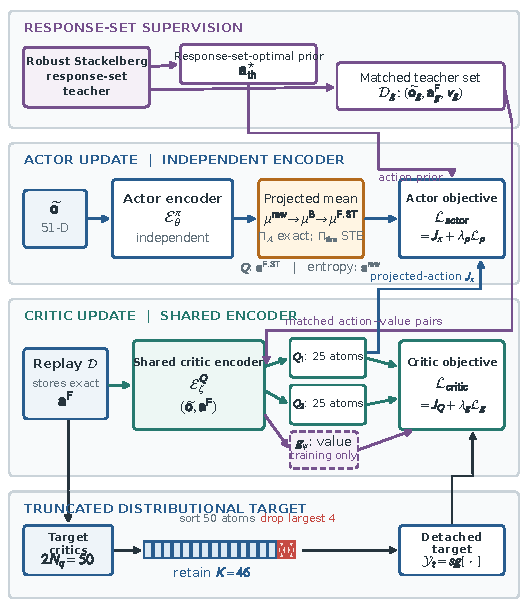
\includegraphics[width=\columnwidth]{tqc_network_diagram.pdf}
\caption{Response-set-guided projected-action TQC training. The actor uses an
independent encoder and receives the response-set-optimal action prior. The
two quantile heads and the training-only robust-value head share the critic
encoder, while matched samples in $\mathcal D_g$ supervise their corresponding
projected actions. The largest four target atoms are discarded before the
detached critic backup.}
\label{fig:tqc_network}
\end{figure}

\subsection{Persistent intention and corridor synthesis}
\label{subsec:corridor_synthesis}
The state machine carries the selected passing opportunity across successive
tactical updates. This temporal persistence complements the spatial corridor:
the policy may refine its width and speed request as the encounter evolves,
while the committed side remains consistent through the pass.
Let $g_t$ and $\Delta v_t$ be the sampled relative quantities defined in
Eq.~\eqref{eq:rel}.
A feasible side is committed as the ego closes on the opponent, retained
through \textsc{Shadow} and \textsc{Overtake}, and released only after a
confirmed pass, an abort, or an execution-health failure. Health and abort
take precedence over passing, completed passes take precedence over continued
overtaking, and an unlocked ego enters \textsc{Defend} only when a rear
opponent is closing. The post-pass indicator $P_t$ used in the reward denotes
$N_{\rm post}$ consecutive updates beyond the overtake clearance threshold.

The geometric operation that realizes the selected side is the corridor
carver. For $\mathcal B_{{\rm cap},k}=[\ell_k,u_k]$, the vehicle footprint and
one-sided exclusion are
\begingroup
\setlength{\arraycolsep}{2pt}
\begin{equation}
\begin{aligned}
\rho_{{\rm exc},k}&=d_{\rm safe}+\frac12\sum_{j\in\{e,o\}}
(L_j|\sin\xi_{j,k}|+W_j|\cos\xi_{j,k}|),\\
\mathcal B_{{\rm cap},k}&=
[\max\{n_{{\rm trk},k}^{-},-R^{\rm cap}\},
\min\{n_{{\rm trk},k}^{+},L^{\rm cap}\}],\\
\mathcal C_k^{\rm side}(\sigma,\eta)&=\begin{cases}
[\ell_k+\eta[n_{o,k}+\rho_{{\rm exc},k}-\ell_k]_+,u_k],&\sigma=+1,\\
[\ell_k,u_k-\eta[u_k-n_{o,k}+\rho_{{\rm exc},k}]_+],&\sigma=-1.
\end{cases}
\end{aligned}
\label{eq:core_overtake_carver}
\end{equation}
\endgroup
Here $\sigma=+1$ and $-1$ select the left and right passing sides,
respectively. \textsc{Shadow} uses
$\eta=\operatorname{clip}((g_{\rm chase}-\widehat g_k)/
(g_{\rm chase}-g_{\rm ot}),0,1)$, whereas \textsc{Overtake} uses full
exclusion ($\eta=1$) on the locked side. \textsc{Raceline} uses the capped
track interval; \textsc{Defend} intersects it with a width-$w_{\rm safe}$
interval centred at the clipped offset $n_{o,k}+b_{\rm lat}$; and
\textsc{Hold} retains only the connected component containing the ego vehicle.
Figure~\ref{fig:tactical_mode_semantics} illustrates these geometric semantics.

\begin{figure}[!tbp]
\centering
\subfloat[\textrm{\textsc{Raceline}/\textsc{Hold}}.]{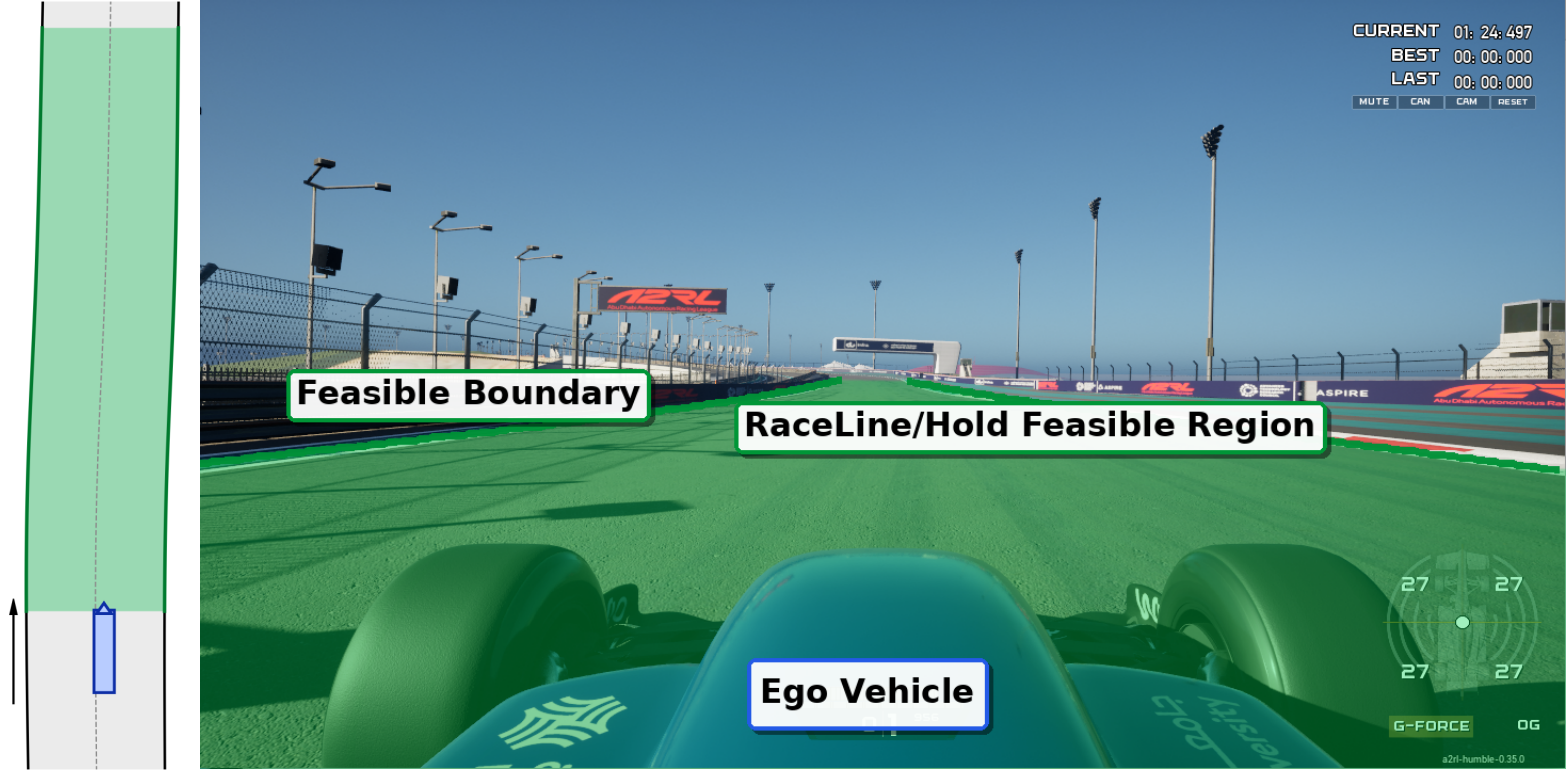
\includegraphics[width=0.48\linewidth]{race.png}}
\hfill
\subfloat[\textrm{\textsc{Shadow}}.]{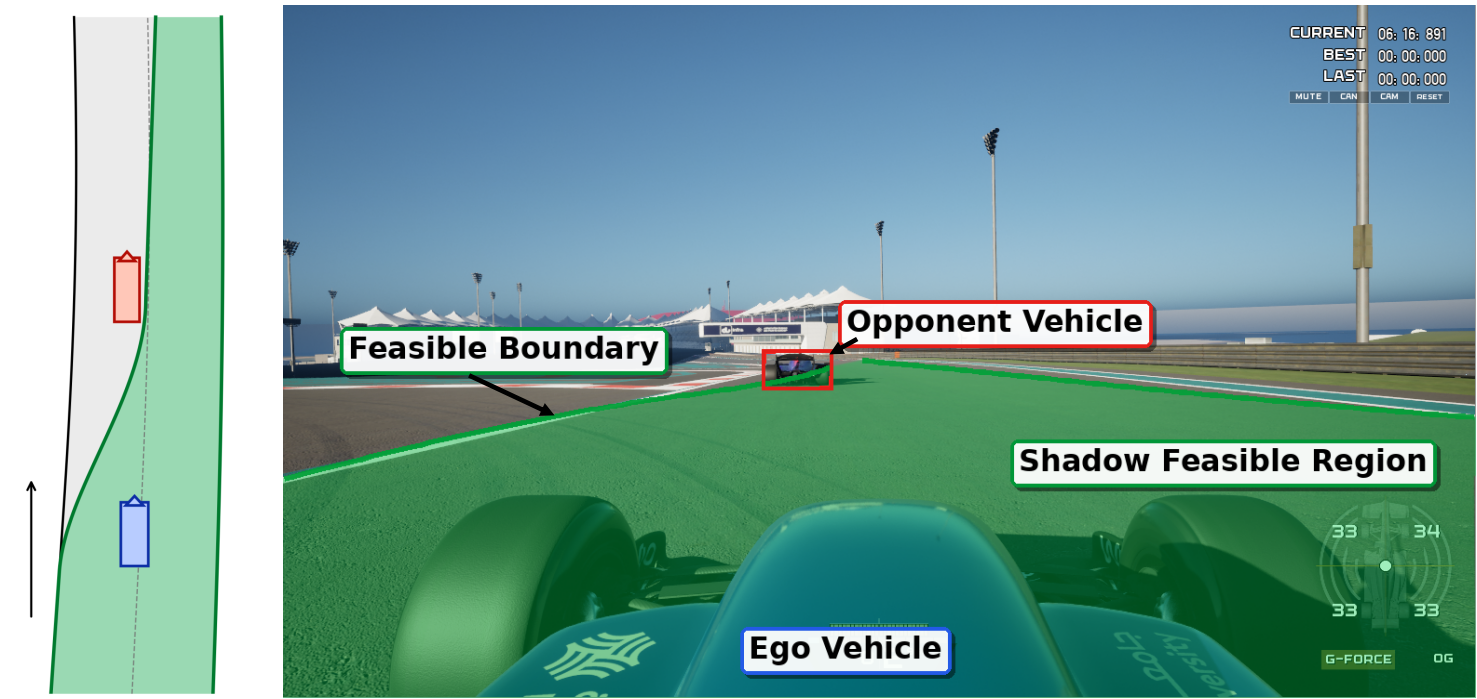
\includegraphics[width=0.48\linewidth]{shadow.png}}\\[-1mm]
\subfloat[\textrm{\textsc{Overtake}}.]{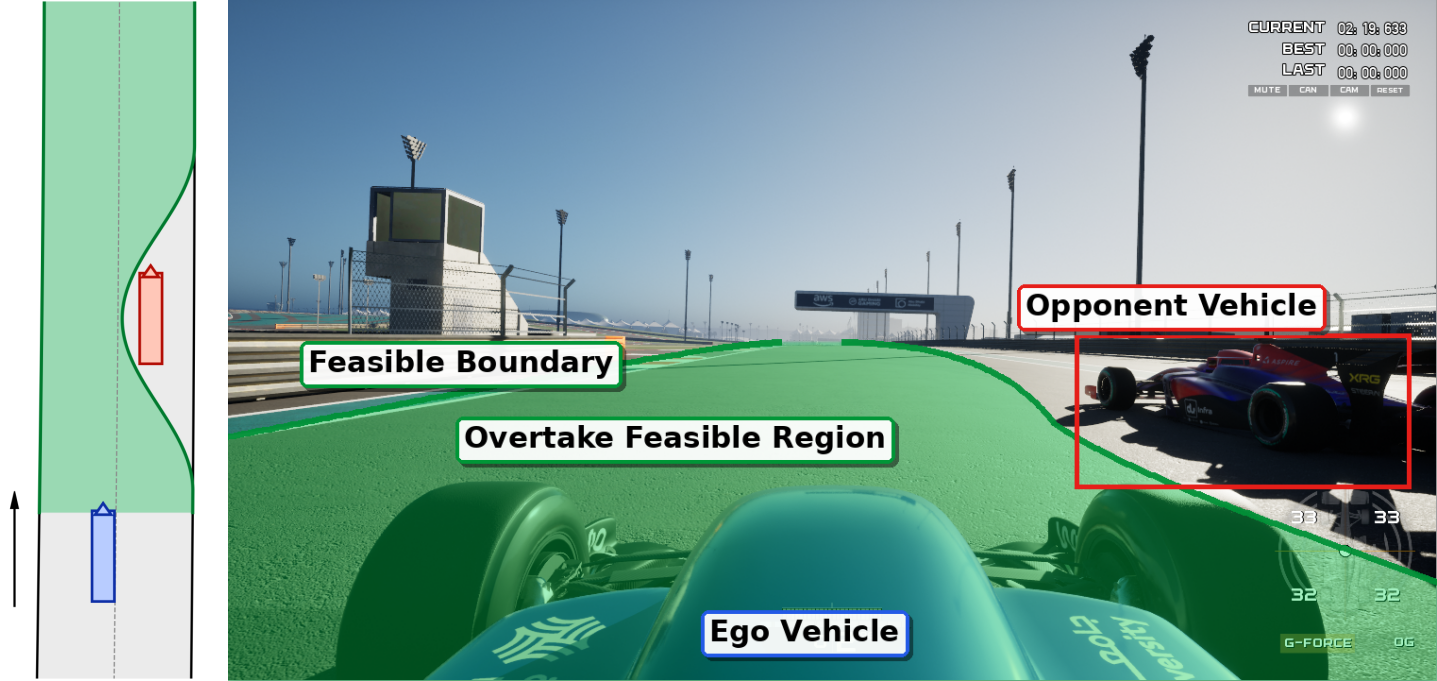
\includegraphics[width=0.48\linewidth]{overtake.png}}
\hfill
\subfloat[\textrm{\textsc{Defend}}.]{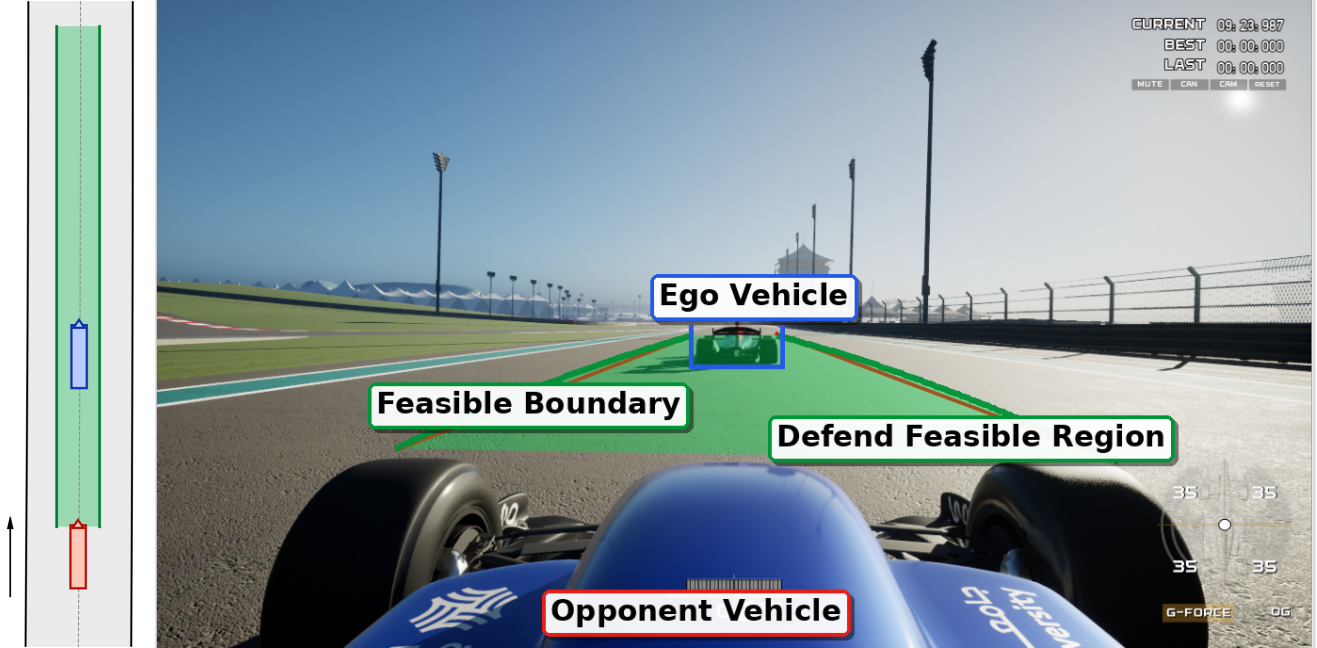
\includegraphics[width=0.48\linewidth]{defend.png}}
\caption{Nominal geometry of the persistent tactical modes. Each panel pairs
the Frenet feasible region with the corresponding simulator view; the shaded
interval is the region delivered to the planner.}
\label{fig:tactical_mode_semantics}
\end{figure}

Algorithm~\ref{alg:tactical_corridor} summarizes the complete route from
offline interaction supervision to online corridor publication. Immediate
contraction and smoothed relaxation allow the feasible region to respond
quickly to reduced space while expanding progressively as the passing channel
opens. The preceding corridor is revalidated for one update when a new
interval loses the required width.

\begin{algorithm}[!tbp]
\caption{Game-supervised tactical-corridor policy}
\label{alg:tactical_corridor}
\footnotesize
\begin{algorithmic}[1]
\REQUIRE teacher states and replay $\mathcal D$; online states, track preview,
previous $(m,\sigma^{\rm lock},\mathcal C)$, and execution health
\STATE \textbf{Offline teacher and training:}
\FOR{each teacher state}
\STATE combine Sobol samples with left/neutral/right codes; apply
$\bm a^{\rm raw}\!\rightarrow\!\bm a^{\rm B}\!\rightarrow\!\bm a^{\rm F}$
\STATE discard duplicate or infeasible candidates; generate the coupled
preview~\eqref{eq:coupled_game_preview} for each candidate pair
\STATE evaluate~\eqref{eq:game_utility}, retain near-best follower responses,
and compute~\eqref{eq:response_set_teacher}
\STATE store every matched
$(\widetilde{\bm o},\bm a^{\rm F},v_g,\bm a_{\rm th}^{\star})$
in $\mathcal D_g$
\ENDFOR
\STATE update TQC from $\mathcal D$ and the prior/value terms from $\mathcal D_g$
using Eq.~\eqref{eq:total_loss}
\STATE \textbf{Online tactical publication:}
\STATE sample $\bm a^{\rm raw}$, apply $\Pi_{\mathcal A}$, predict the opponent
at constant Frenet velocity, and evaluate the available side widths
\IF{$h_t$ is invalid, or a locked state satisfies $g_t\ge g_{\rm abort}$ or
loses $L_{\min}^{\rm corr}$ width}
\STATE set \textsc{Hold} and release the side lock
\ELSIF{the locked ego satisfies $g_t\le-g_{\rm ot}$ for $N_{\rm post}$ updates}
\STATE set $P_t=1$, return to \textsc{Raceline}, and release the lock
\ELSIF{a lock exists, or a non-neutral feasible side is requested with
$0<g_t\le g_{\rm chase}$ and $\Delta v_t\ge0$}
\STATE retain/commit that side; select \textsc{Shadow} for $g_t>g_{\rm ot}$
and \textsc{Overtake} otherwise
\ELSIF{$\sigma^{\rm lock}=0$, $-g_{\rm chase}\le g_t<0$, and
$\Delta v_t<0$}
\STATE select \textsc{Defend}
\ELSE
\STATE select \textsc{Raceline}
\ENDIF
\STATE construct the mode interval using~\eqref{eq:core_overtake_carver} and
the corresponding raceline, defend, or connected-hold rule; use
$\eta=1$ in \textsc{Overtake} and the gap-based ramp in \textsc{Shadow}
\STATE evaluate~\eqref{eq:tire_safe_action}, including its deterministic
current-state \textsc{Hold}/braking branch
\STATE apply immediate contraction and smoothed relaxation; on width failure,
revalidate the preceding corridor for at most one update
\RETURN $(m,\sigma^{\rm lock},V_{\rm cap}^{\rm F},\mathcal C)$ if valid;
otherwise return braking-fallback status
\end{algorithmic}
\end{algorithm}

% =====================================================================
\section{Corridor-Constrained Planning and Reference Tracking}
\label{sec:execution}\label{sec:planner}\label{sec:controller}
% =====================================================================

The execution layer realizes the persistent tactical feasible region as a
continuous path--speed reference and actuator commands. The published corridor
defines the spatial optimization domain, while the speed request sets the
tactical pace throughout the maneuver. At station \(s_k\),
\([\underline n_k,\overline n_k]\) is the footprint-eroded vehicle-center
interval. Sequential iteration \(j\) linearizes Eq.~\eqref{eq:spatial_model} as
\(\widehat{\bm f}_{s,k}^{j}=\bm A_k^j\bm z_k+\bm B_k^j\omega_k+\bm b_k^j\)
and solves one corridor-constrained SOCP subproblem:
\begingroup
\setlength{\arraycolsep}{2pt}
\small
\begin{equation}
\begin{aligned}
\bm y^{j+1}=\argmin_{\bm y}\;&
\sum_kw_\omega\sigma_k^\omega
+w_{n,T}\epsilon_n+w_{\xi,T}\epsilon_\xi\\
\mathrm{s.t.}\;&\bm z_0=[n_e,\xi_e]^\top,\quad
 \bm z_{k+1}-\bm z_k=\frac{\Delta s_{\rm sta}}{2}
 (\widehat{\bm f}_{s,k}^{j}+\widehat{\bm f}_{s,k+1}^{j}),\\
&\underline n_k\le n_k\le\overline n_k,\quad
1-\kappa(s_k)n_k\ge\varepsilon_s,\\
&|\xi_k|\le\xi_{\max},\quad |\omega_k|\le\omega_{\max},\\
&\left\|[2\omega_k,\sigma_k^\omega-1]^\top\right\|_2
\le\sigma_k^\omega+1,\\
&|n_{N-1}-n_T|\le\epsilon_n,\quad
|\xi_{N-1}-\xi_T|\le\epsilon_\xi,\quad
\epsilon_n,\epsilon_\xi\ge0 .
\end{aligned}
\label{eq:execution_socp}
\end{equation}
\endgroup
Here \(\bm y=\{\bm z_k,\omega_k,\sigma_k^\omega,\epsilon_n,\epsilon_\xi\}\),
\(\bm z_k=[n_k,\xi_k]^\top\), and
\(\omega_{\max}=\tan\delta_{\max}/(l_f+l_r)\).
The terminal target is the clipped raceline in \textsc{Raceline} and the
corridor midpoint otherwise, with \(\xi_T=0\). The conic epigraph penalizes
path curvature, and the terminal slacks soften convergence to
$(n_T,0)$. The nonlinear Frenet model is re-evaluated after each sequential
update.

The forward--backward sweep distributes the certified tactical cap over the
optimized path.
For curvature \(\kappa_{p,k}\), the envelope supplies the traction and
braking limits \(a_{T,k}^{+}\) and \(b_{T,k}^{-}\) at
\((\kappa_{p,k}V^2,V)\), after subtracting the resistance acceleration in
traction and adding it in braking.
The steady tactical request is first converted into a braking-reachable
stationwise cap $V_{{\rm cap},k}^{\rm P}$. Intersecting it with the largest
envelope-admissible curvature speed gives
$V_{{\rm lim},k}=\min\{\overline V_{{\rm curv},k},
V_{{\rm cap},k}^{\rm P}\}$. The resulting forward--backward sweep is
\begin{equation}
\begin{aligned}
V_0^f&=V_e,\\
V_{k+1}^{f}&=\operatorname{clip}_{[V_{\min},V_{{\rm lim},k+1}]}
\sqrt{(V_k^f)^2+2\Delta\ell_k a_{T,k}^{+}(V_k^f)},\\
V_{N-1}^r&=\min\{V_{N-1}^{f},V_{{\rm lim},N-1}\},\\
V_k^r&=\min\left\{V_k^f,V_{{\rm lim},k},
\sqrt{(V_{k+1}^r)^2+
2\Delta\ell_k b_{T,k+1}^{-}(V_{k+1}^r)}\right\}.
\end{aligned}
\label{eq:execution_speed_sweep}
\end{equation}
The forward pass starts at the measured speed, whereas the backward pass
enforces downstream braking reachability. Trapezoidal integration of
$1/V_k^r$ provides the time stamps used to resample the path--speed reference
on the controller grid.

The RC-NMPC tracks the resampled path--speed reference on a fixed prediction
grid. Its state and input are $\bm\chi_k=[x_k,y_k,\theta_k]^\top$ and
$\bm\nu_k=[V_k,\delta_k]^\top$, respectively. The controller solves
\begin{equation}
\begin{aligned}
\min_{\{\bm\nu_k\}}\;&q_{\Delta\delta}(\delta_0-\delta_{-1})^2+
\sum_{k=0}^{N_c-1}\!\left(q_ce_{c,k+1}^2+q_\psi e_{\psi,k+1}^2\right.\\[-1mm]
&\left.\hspace{26mm}+\bm e_{\nu,k}^\top\bm R_\nu\bm e_{\nu,k}\right)\\
\mathrm{s.t.}\;&\bm\chi_0=\bm0,\quad
\bm\chi_{k+1}=\bm\chi_k+T_c
\begin{bmatrix}
V_k\cos\theta_k\\ V_k\sin\theta_k\\
V_k\tan\delta_k/(l_f+l_r)
\end{bmatrix},\\
&V_{\min}\le V_k\le
\min\{v_{x,\max},V_{{\rm cap},t,k}^{\rm C}\},\\
&|\delta_k|\le\delta_{\max},\quad
|V_k-V_{k-1}|\le\Delta V_{\max},\\
&|\delta_k-\delta_{k-1}|\le\dot\delta_{\max}T_c .
\end{aligned}
\label{eq:execution_mpcc}
\end{equation}
Here $\bm\nu_k^r=[V_k^r,\delta_k^r]^\top$, with
$\delta_k^r=\arctan((l_f+l_r)\kappa_{p,k}^r)$. The quantities
$e_{c,k}=(\bm n_k^r)^\top(\bm p_k-\bm p_k^r)$,
$e_{\psi,k}=\operatorname{wrap}(\theta_k-\theta_k^r)$, and
$\bm e_{\nu,k}=\bm\nu_k-\bm\nu_k^r$ are the contouring, heading, and input
tracking errors. The stagewise bound $V_{{\rm cap},t,k}^{\rm C}$ is obtained by
rate-limiting the steady tactical request from the previous speed command.
Realized tire demand is reported in Section~\ref{sec:experiments}.

\begin{algorithm}[!tbp]
\caption{Common reference generator and executor}
\label{alg:executor}
\footnotesize
\begin{algorithmic}[1]
\REQUIRE guidance \(\mathcal G_t\), current state, previous valid reference
\STATE erode the track by the ego footprint, intersect it with $\mathcal C_t$,
and choose the mode-dependent terminal target
\STATE initialize the spatial path from the previous valid solution or the
corridor midpoint
\FOR{each configured sequential-convexification iteration}
\STATE solve SOCP~\eqref{eq:execution_socp}, update the linearization, and
evaluate the nonlinear Frenet and corridor residuals
\STATE stop when the solver and residual tolerances in
\ref{app:parameters} are satisfied
\ENDFOR
\STATE set valid if the path passes the solver, domain, and residual checks
\IF{valid}
\STATE query $\mathcal A_{\rm tire}(V)$ and construct
$V_{{\rm cap},k}^{\rm P}$ from $V_{\rm cap}^{\rm F}$, measured speed, and
available braking
\STATE intersect $V_{{\rm cap},k}^{\rm P}$ with the curvature-speed envelope,
run~\eqref{eq:execution_speed_sweep}, and update valid from the tire check
\ENDIF
\IF{valid}
\STATE time-resample the path--speed reference and rate-limit
$V_{{\rm cap},t}^{\rm F}$ to obtain $V_{{\rm cap},t,k}^{\rm C}$
\STATE solve RC-NMPC~\eqref{eq:execution_mpcc} and update valid from its status
\ENDIF
\IF{valid}
\STATE map $(V_{0|t}^{c\star},\delta_{0|t}^{c\star})$ to throttle, brake,
steering, and gear
\ELSE
\STATE revalidate the previous reference for one cycle; otherwise request
current-state \textsc{Hold} and issue rate-limited braking with the preceding
steering angle
\ENDIF
\RETURN four-channel command and health status
\end{algorithmic}
\end{algorithm}
\FloatBarrier
\endgroup
\section{Experimental results and discussion}\label{sec:experiments}
% =====================================================================

\subsection{Experimental platform and configuration}
\label{subsec:hil_env}\label{subsec:param_setup}

The Abu Dhabi Autonomous Racing League (A2RL) provides a full-scale
head-to-head racing environment in which EAV24 vehicles compete autonomously
at the Yas Marina Circuit. We reproduced this operating chain in a
target-hardware HIL platform (Fig.~\ref{fig:a2rl_sim}). The AutoVerse EAV24
plant and track environment ran on a simulation server and generated radar,
GNSS/IMU, wheel-speed, and race-control data. These streams reached the Neousys
RGS-8805GC onboard computer over a dedicated Ethernet link using DDSI--RTPS
over UDP/IP. The tactical, planning, and control modules executed on the target
computer, which returned throttle, brake, steering, and gear commands to the
simulated vehicle through CAN.

\begin{figure}[!tbp]
\centering
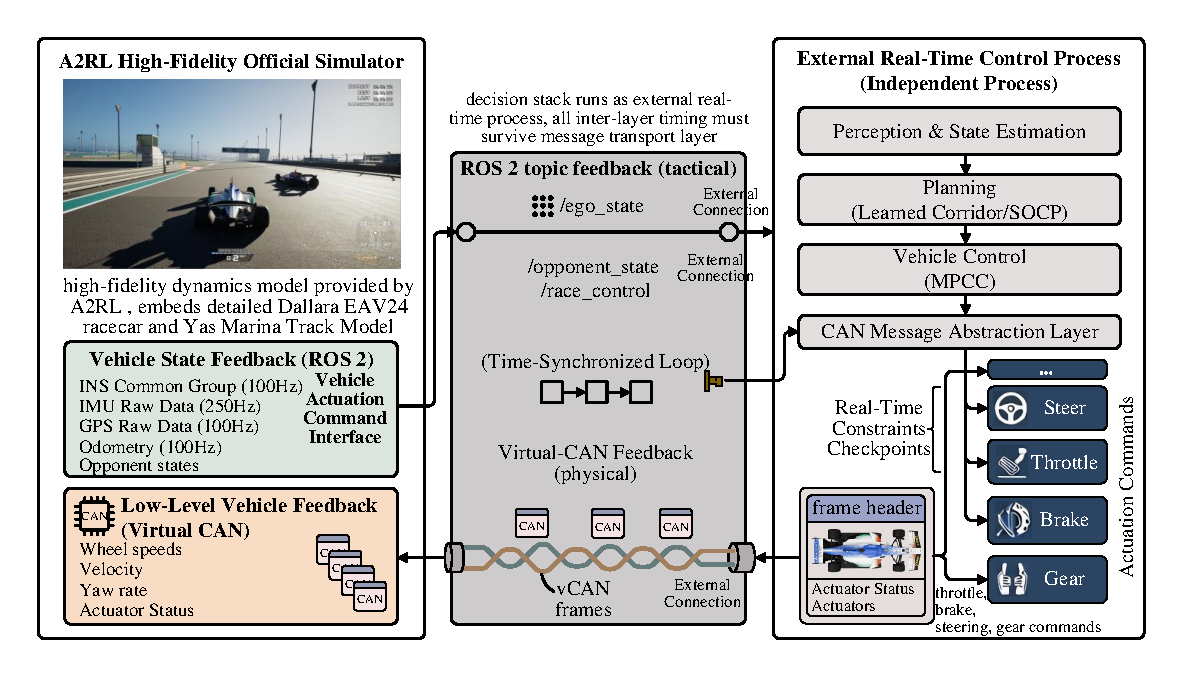
\includegraphics[width=\linewidth]{sim_shuoming.pdf}
\caption{Target-hardware HIL topology. The AutoVerse server publishes radar,
GNSS/IMU, wheel-speed, and race-control data to the RGS-8805GC over Ethernet
using DDSI--RTPS over UDP/IP; the target computer returns throttle, brake,
steering, and gear commands to the EAV24 vehicle model through CAN.}
\label{fig:a2rl_sim}
\end{figure}

Ego position, velocity, attitude, and acceleration are delivered at 100~Hz
with the configured localization noise and latency. Opponent perception is
updated at 20~Hz with radar range-noise base/scale values of 0.02/0.003,
0.003-rad azimuth noise, a 0.22 velocity-noise scale, a 10\% packet-drop rate,
and front/left/right/rear time offsets of 0/40/40/20~ms. The decision and
planning modules run at 50~Hz, and the control module outputs throttle, brake,
steering, and gear commands at 100~Hz.

Statistical results aggregate 1000 Monte Carlo closed-loop simulations per
setting. OSR is the fraction of completed overtakes, and TTO is their completion
time. Minimum gap, mean TTC, and contact/track-violation rates describe
interaction safety, while PFR is the fraction of feasible planning updates.

\subsection{Overtaking performance under representative track conditions}
\label{subsec:representative_cases}

To examine whether the learned feasible region remains coherent across
different overtaking geometries, Fig.~\ref{fig:four_case_track_overview}
presents four encounters at separated locations on the Yas Marina circuit.
Each spatial view pairs the published corridor and planned path with
synchronized \textsc{Shadow} and \textsc{Overtake} frames. Cases~I and II are
then examined in detail as complementary examples of short-window high-speed
commitment and persistent passing through a sharp-corner sequence.

\begin{figure*}[!t]
\centering
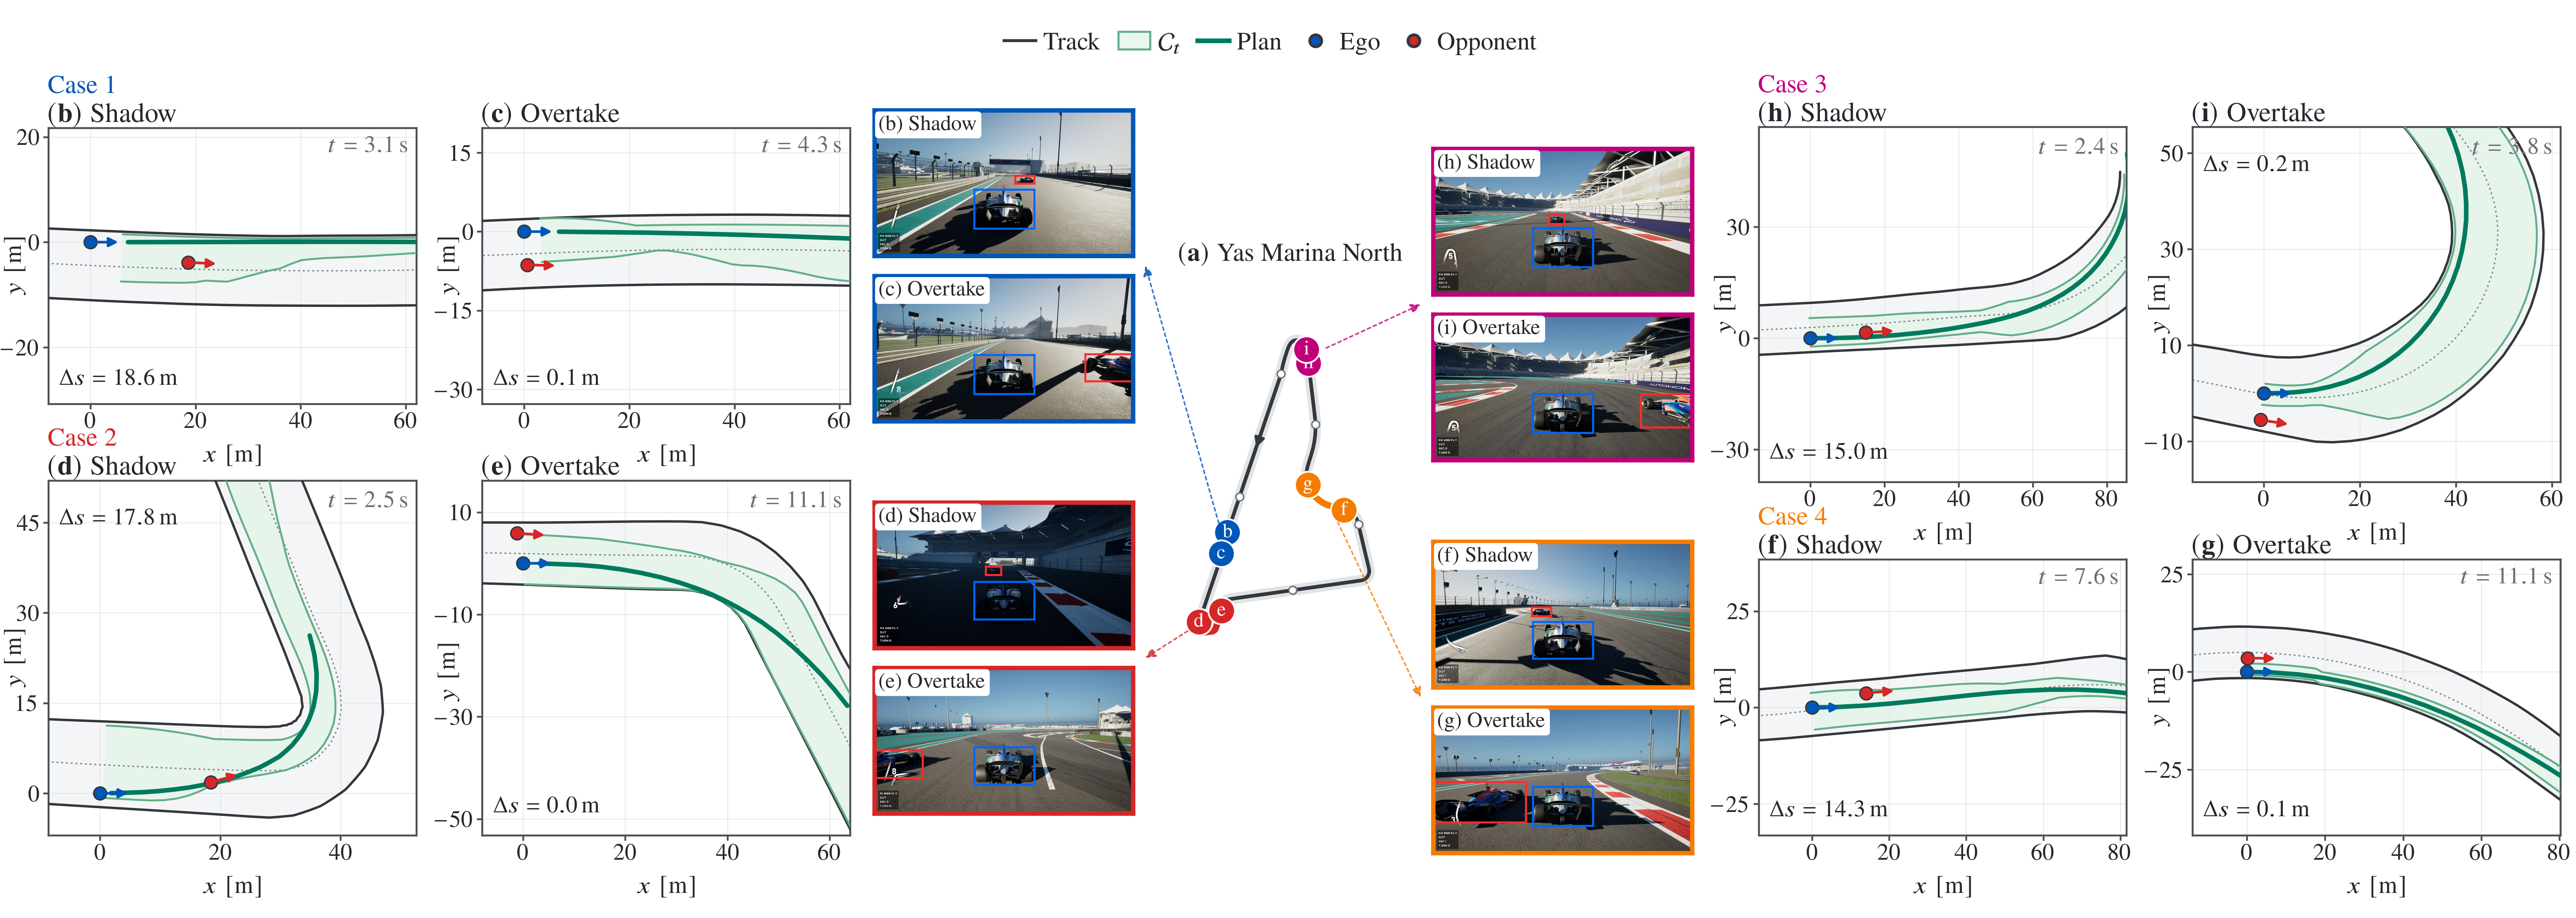
\includegraphics[width=\textwidth]{track_overview_case0205_v018.png}
\caption{Representative overtaking situations on the Yas Marina circuit. Each
colored location links the spatial corridor and planned path to synchronized
\textrm{\textsc{Shadow}} and \textrm{\textsc{Overtake}} simulator views.}
\label{fig:four_case_track_overview}
\end{figure*}

\subsubsection*{Case I: high-speed overtake with a short commitment window}

Case~I begins near 69~m~s$^{-1}$ with a substantially slower opponent and a
short commitment window. Figure~\ref{fig:case02_tactical_new} shows the ordered
transition from \textsc{Raceline} through \textsc{Shadow} to
\textsc{Overtake}. The side-locked corridor forms a continuous lateral channel
inside the physical track boundaries, and the optimized ego path follows this
channel while establishing separation from the opponent. The actual speed
tracks the desired profile and exceeds 70~m~s$^{-1}$ during the pass, showing
that the tactical opportunity is preserved through high-speed execution.

\begin{figure}[!tbp]
\centering
\subfloat[FSM mode sequence.]{
\includegraphics[width=\linewidth]{other_pic_V18/single_panels/case_02_fsm_mode.png}}\\[-0.5mm]
\subfloat[Path, corridor, and track bounds.]{
\includegraphics[width=\linewidth]{other_pic_V18/single_panels/case_02_path_corridor.png}}\\[-0.5mm]
\subfloat[Vehicle-speed response.]{
\includegraphics[width=\linewidth]{other_pic_V18/single_panels/case_02_dynamics_speed.png}}
\caption{Tactical and speed evolution in Case~I. (a) The FSM establishes a
persistent passing phase. (b) The planned path remains inside the published
corridor and physical track boundaries. (c) The actual speed tracks the desired
profile above 70~m~s$^{-1}$ while closing on the opponent.}
\label{fig:case02_tactical_new}
\end{figure}

Figure~\ref{fig:case02_tracking_new} shows the closed-loop realization of this
passing channel. Lateral, speed, and heading errors remain concentrated around
zero, with brief transients during the tactical transition, and the complete
acceleration sequence remains inside the speed-dependent tire-demand envelope.
The spatial decision therefore propagates from side commitment to a trackable
path--speed reference throughout the high-speed pass.

\begin{figure}[!tbp]
\centering
\subfloat[Lateral contouring error.]{
\includegraphics[width=\linewidth]{other_pic_V18/single_panels/case_02_tracking_lateral.png}}\\[-0.5mm]
\subfloat[Speed-tracking error.]{
\includegraphics[width=\linewidth]{other_pic_V18/single_panels/case_02_tracking_speed.png}}\\[-0.5mm]
\subfloat[Heading-tracking error.]{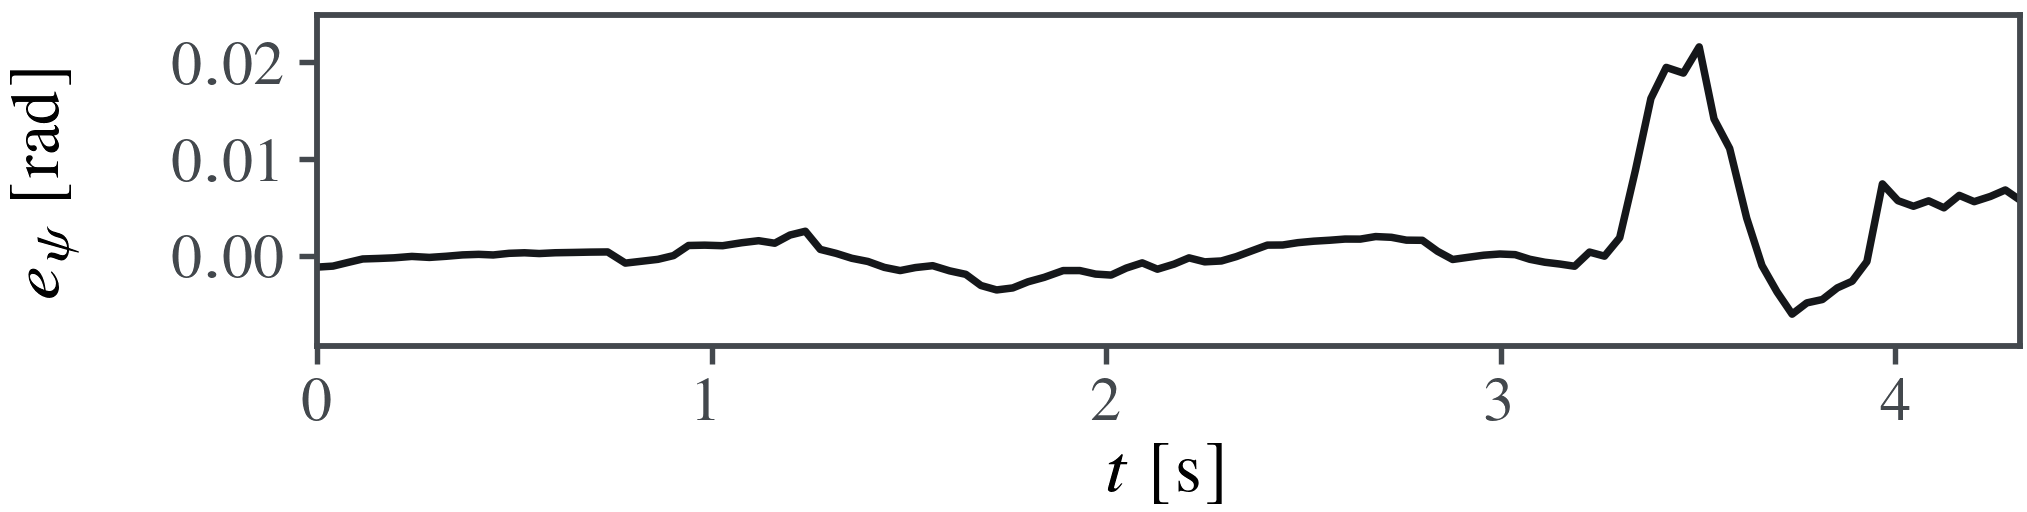
\includegraphics[width=\linewidth]{other_pic_V18/single_panels/case_02_tracking_heading.png}}\\[-0.5mm]
\subfloat[Realized acceleration demand.]{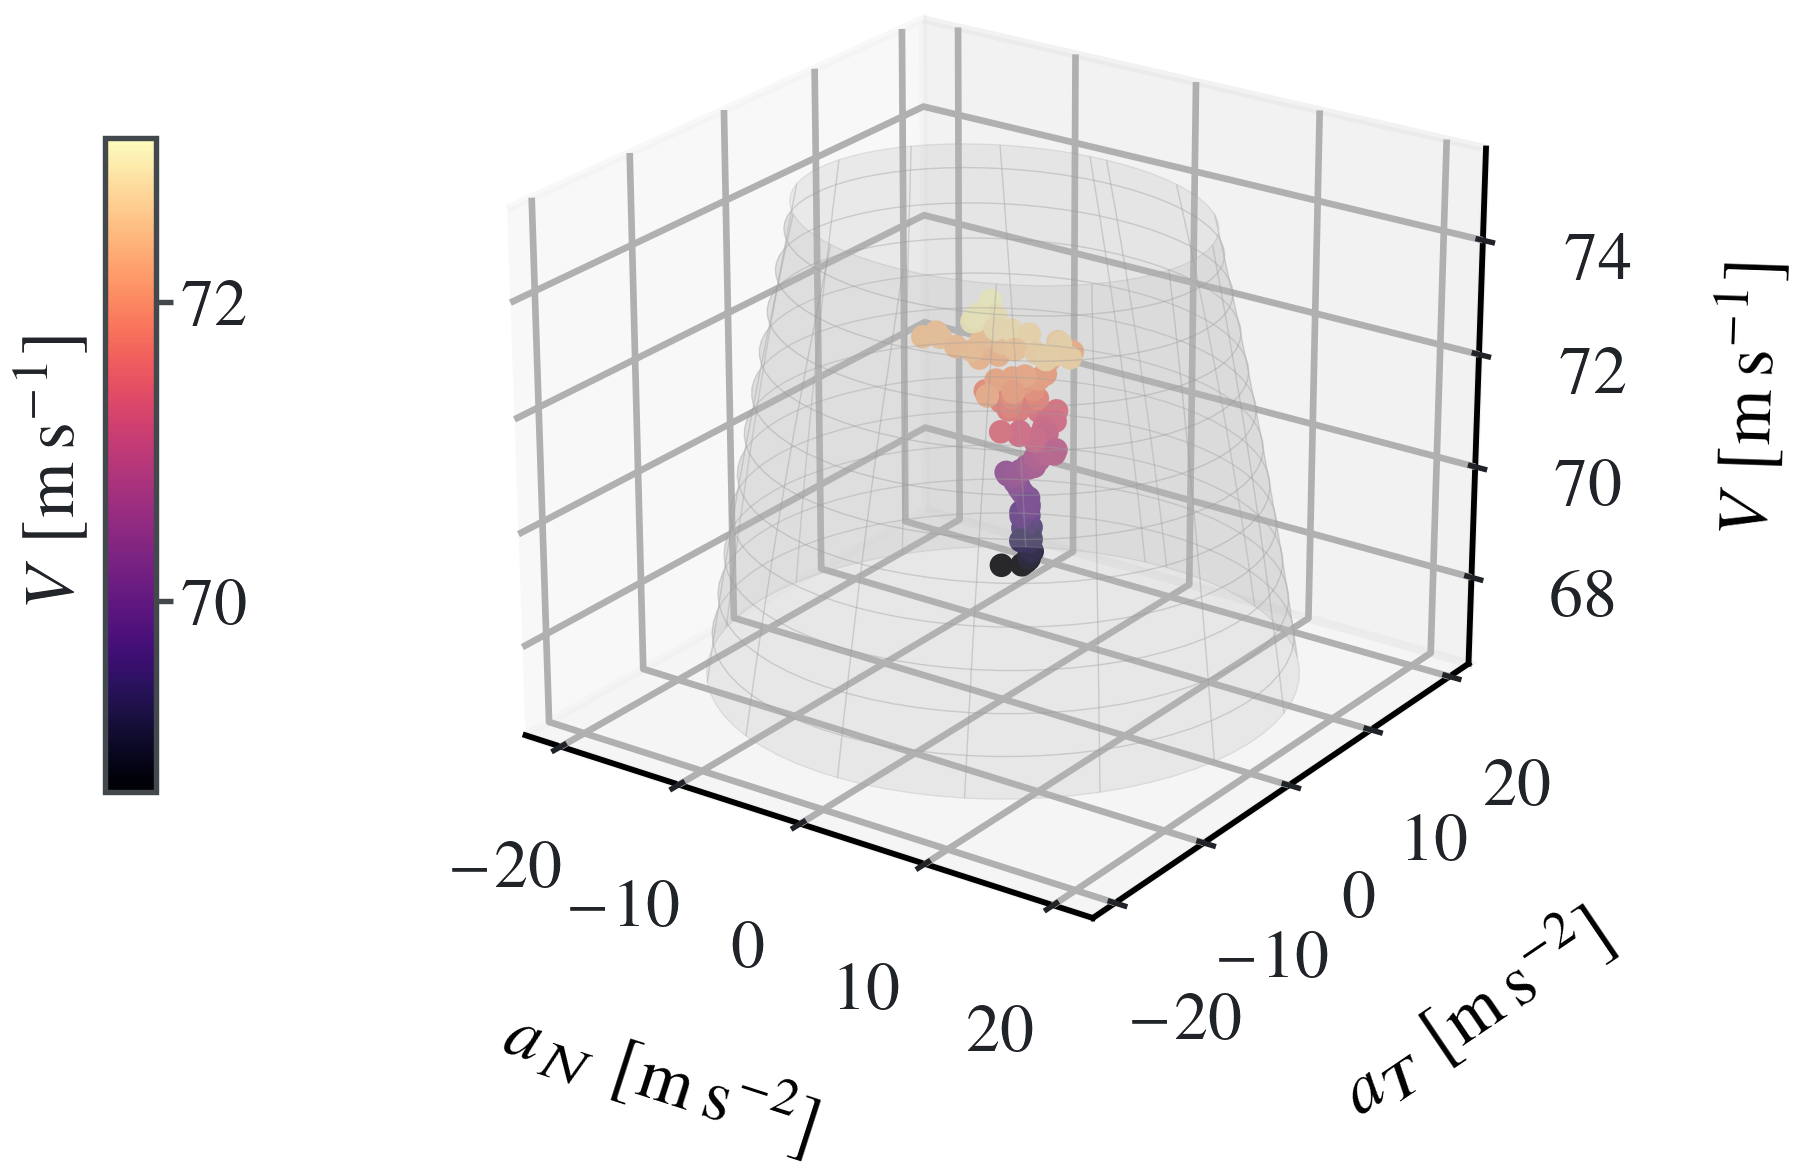
\includegraphics[width=\linewidth]{other_pic_V18/single_panels/case_02_gg_diagram.png}}
\caption{Closed-loop tracking and tire-demand response in Case~I. (a--c)
Lateral, speed, and heading errors remain bounded through the tactical
transition and pass. (d) All recorded tangential--normal acceleration samples
remain inside the declared speed-dependent tire-demand envelope.}
\label{fig:case02_tracking_new}
\end{figure}

\subsubsection*{Case II: persistent overtake through a sharp-corner sequence}

Case~II combines an entry speed above 60~m~s$^{-1}$ with a longer interaction
through successive curvature changes. Figure~\ref{fig:case05_tactical_new}
shows that the FSM establishes \textsc{Shadow} and then retains
\textsc{Overtake} through the curved engagement. As the physical track width
changes, the carver continuously reshapes the locked-side corridor and the
planned path remains within the available channel. The speed response follows
the desired braking profile into the corner and the subsequent acceleration
above 35~m~s$^{-1}$, maintaining the passing opportunity throughout the
sequence.

\begin{figure}[!tbp]
\centering
\subfloat[FSM mode sequence.]{
\includegraphics[width=\linewidth]{other_pic_V18/single_panels/case_05_fsm_mode.png}}\\[-0.5mm]
\subfloat[Path, corridor, and track bounds.]{
\includegraphics[width=\linewidth]{other_pic_V18/single_panels/case_05_path_corridor.png}}\\[-0.5mm]
\subfloat[Vehicle-speed response.]{
\includegraphics[width=\linewidth]{other_pic_V18/single_panels/case_05_dynamics_speed.png}}
\caption{Tactical and speed evolution in Case~II. (a) The FSM retains the
selected passing side through the curved engagement. (b) The planned path and
published corridor remain inside the varying physical track boundaries. (c)
The actual speed tracks the desired braking and re-acceleration profile.}
\label{fig:case05_tactical_new}
\end{figure}

The simultaneous braking, turning, and relative-position change produces
larger transient errors than in Case~I
(Fig.~\ref{fig:case05_tracking_new}). Lateral and heading errors return toward
zero after each curvature transition, speed tracking remains bounded during
braking and re-acceleration, and the acceleration samples remain inside the
tire envelope over the recorded speed range. Together, the two cases show that
the learned corridor remains persistent and executable during both a pass
above 70~m~s$^{-1}$ and a constrained corner sequence.

\begin{figure}[!tbp]
\centering
\subfloat[Lateral contouring error.]{
\includegraphics[width=\linewidth]{other_pic_V18/single_panels/case_05_tracking_lateral.png}}\\[-0.5mm]
\subfloat[Speed-tracking error.]{
\includegraphics[width=\linewidth]{other_pic_V18/single_panels/case_05_tracking_speed.png}}\\[-0.5mm]
\subfloat[Heading-tracking error.]{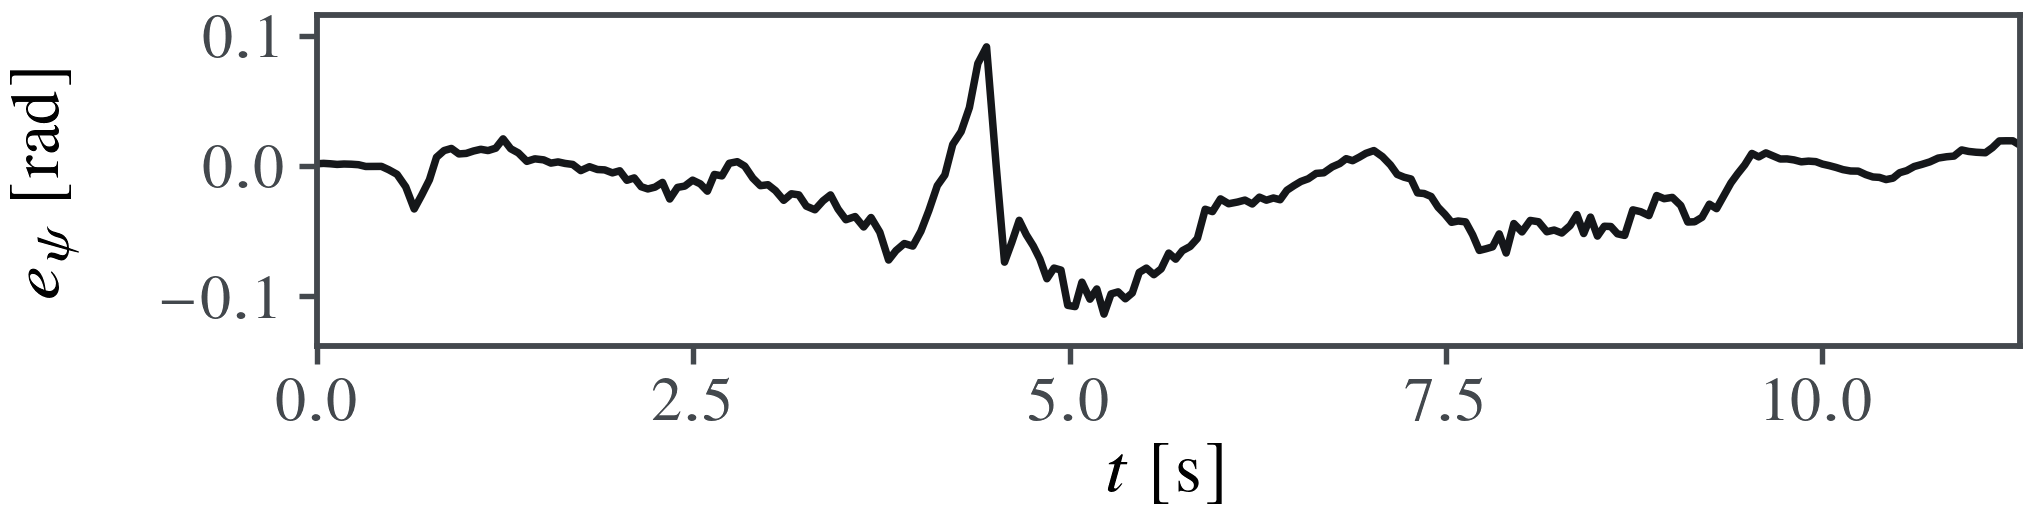
\includegraphics[width=\linewidth]{other_pic_V18/single_panels/case_05_tracking_heading.png}}\\[-0.5mm]
\subfloat[Realized acceleration demand.]{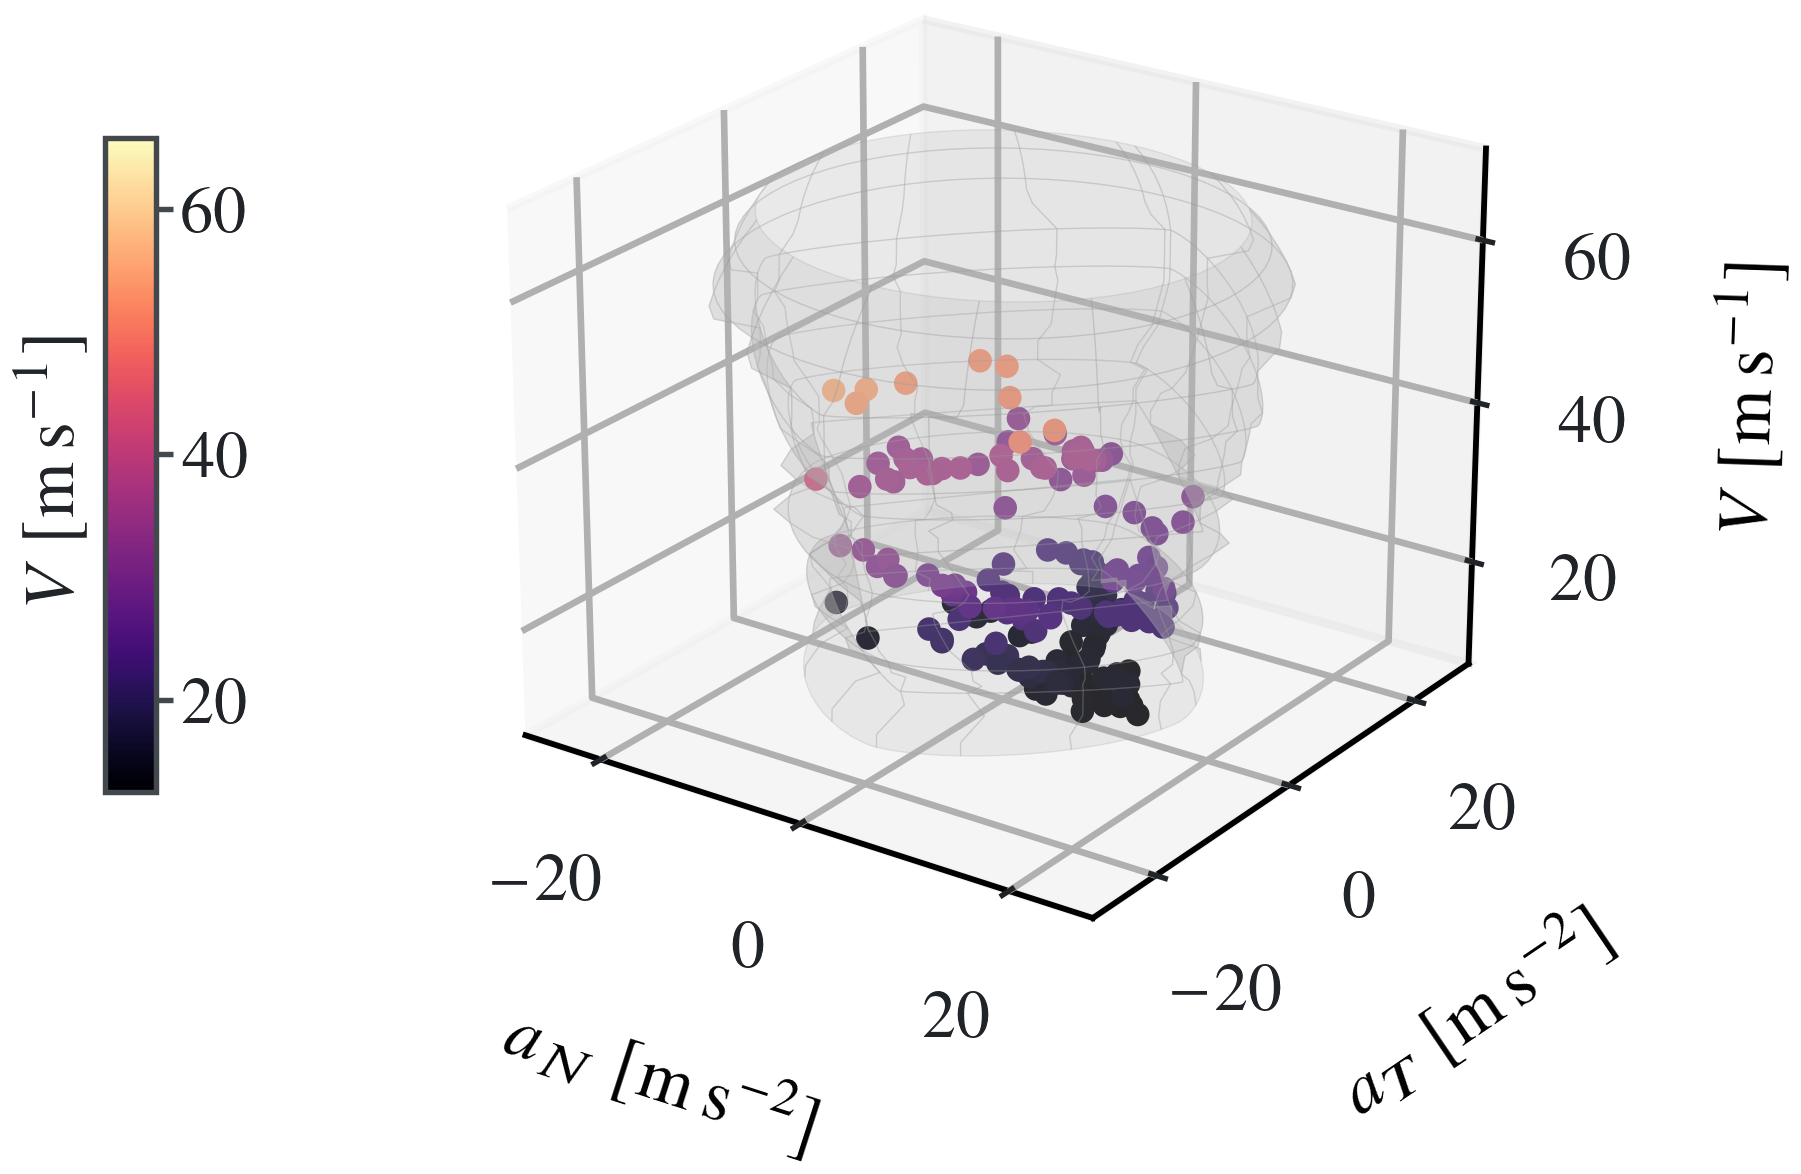
\includegraphics[width=\linewidth]{other_pic_V18/single_panels/case_05_gg_diagram.png}}
\caption{Closed-loop tracking and tire-demand response in Case~II. (a--c)
Tracking remains bounded through the prolonged curved interaction, including
the braking, rotation, and exit phases. (d) All recorded acceleration samples
remain inside the declared speed-dependent tire-demand envelope.}
\label{fig:case05_tracking_new}
\end{figure}

Across 1000 Monte Carlo runs, the full method achieved an OSR of 94.7\%,
with collision and track-violation rates of 0.0\%. The matched
comparisons below quantify the contribution of the interactive tactical
representation and its constituent modules.

% =====================================================================
% Matched comparison and ablation results
% =====================================================================

\subsection{Comparison with tactical baselines}
\label{subsec:comparison}

All methods use the same plant, race-control interface, corridor projection,
path and speed planners, and control module, with the tactical
guidance module defining each comparison. \emph{Pure Raceline} follows the
nominal racing line. \emph{Non-Interactive MPC} predicts the opponent
independently of the ego plan and imposes obstacle constraints on the
result~\cite{kabzan2020amzracing,betz2023autonomous}.
\emph{Rule-based GT} uses a fixed-threshold state machine
($g_{\rm chase}=20$ m, $g_{\rm ot}=8$ m, and $g_{\rm abort}=35$ m).
\emph{iLQGames} computes coupled local responses with iterative
linear-quadratic game approximations~\cite{fridovich2020ilqgames}. Outputs from
all baselines are projected onto the same side, speed-cap, and corridor
interface, yielding a matched comparison of tactical reasoning.

\begin{table}[!tbp]
\centering
\footnotesize
\setlength{\tabcolsep}{2.3pt}
\renewcommand{\arraystretch}{1.08}
\caption{Matched comparison over 1000 Monte Carlo closed-loop HIL runs per
method. Arrows indicate the preferred direction.}
\label{tab:comparison}
\begin{tabular}{@{}lccccc@{}}
\toprule
Metric & Prop. & PR & NI-MPC & RB-GT & iLQG \\
\midrule
OSR [\%] $\uparrow$             & \textbf{94.7} & 38.2 & 28.5 & 51.6 & 63.5 \\
OSR def. [pp] $\downarrow$      & \textbf{0.0} & 56.5 & 66.2 & 43.1 & 31.2 \\
TTO [s] $\downarrow$            & \textbf{4.82} & 7.25 & 11.23 & 9.37 & 7.83 \\
Min. gap [m] $\uparrow$         & \textbf{5.83} & 1.42 & 3.85 & 2.14 & 2.31 \\
Contact [\%] $\downarrow$      & \textbf{0.0} & 2.1 & 0.7 & 4.8 & 1.4 \\
Mean TTC [s] $\uparrow$         & \textbf{8.52} & 3.21 & 6.92 & 5.64 & 5.73 \\
Track viol. [\%] $\downarrow$  & \textbf{0.0} & \textbf{0.0} & \textbf{0.0} & \textbf{0.0} & \textbf{0.0} \\
PFR $\uparrow$                  & \textbf{1.000} & 0.988 & 0.998 & 0.987 & 0.995 \\
\bottomrule
\end{tabular}
\vspace{1mm}

\begin{minipage}{\columnwidth}
\scriptsize
\emph{Notes:} Prop., proposed method; PR, Pure Raceline; NI-MPC,
Non-Interactive MPC; RB-GT, Rule-based GT; iLQG, iLQGames. OSR def.
is the percentage-point deficit from Prop. Min. gap is the mean per-lap
minimum inter-vehicle distance. PFR is the fraction of planning cycles with a
feasible SOCP solution. Bold denotes the best observed value; equal track
violation values are jointly bold.
\end{minipage}
\end{table}

The proposed tactical-corridor policy completed 94.7\% of the laps, exceeding
the strongest baseline, iLQGames, by 31.2 percentage points while increasing
the mean minimum gap from 2.31 to 5.83~m and reducing the contact rate from
1.4\% to 0.0\% (Table~\ref{tab:comparison}). iLQGames achieved the strongest baseline result,
showing the value of coupled interaction reasoning, whereas the additional
conversion of that reasoning into a persistent feasible region markedly
increased successful closed-loop realization. The PFR of 1.000 further shows
that the published corridors consistently supplied usable domains to the
common planner across the evaluated laps.

\subsection{Ablation study}
\label{subsec:ablation}

Four ablations isolate the proposed tactical components while retaining the
same execution layer. \emph{Without game guidance} removes both the Stackelberg
response-set action prior and the action-conditioned robust-value supervision.
\emph{Without FSM} bypasses
hysteretic mode and side locking, allowing the policy to reshape the corridor
on every update. \emph{Without learned corridor} replaces the continuous
width, clearance, lateral-bias, and speed-cap outputs by fixed nominal values.
The final variant replaces TQC with Soft Actor-Critic (SAC) while preserving
the network, replay, reward, and other training settings.

\begin{table}[!htbp]
\centering
\footnotesize
\setlength{\tabcolsep}{2.3pt}
\renewcommand{\arraystretch}{1.08}
\caption{Component ablations over 1000 Monte Carlo closed-loop HIL runs per
variant. Each variant removes or replaces one tactical component. Arrows
indicate the preferred direction.}
\label{tab:ablation}
\begin{tabular}{@{}lccccc@{}}
\toprule
Metric & Full & No-GG & No-FSM & Fixed-C & SAC \\
\midrule
OSR [\%] $\uparrow$            & \textbf{94.7} & 85.4 & 82.3 & 76.1 & 88.5 \\
OSR loss [pp] $\downarrow$    & \textbf{0.0} & 9.3 & 12.4 & 18.6 & 6.2 \\
TTO [s] $\downarrow$           & \textbf{4.82} & 6.38 & 6.71 & 8.94 & 5.53 \\
Contact [\%] $\downarrow$    & \textbf{0.0} & 0.9 & 1.2 & 3.1 & 0.5 \\
Min. gap [m] $\uparrow$       & \textbf{5.83} & 2.86 & 2.17 & 1.05 & 3.94 \\
Mean TTC [s] $\uparrow$       & \textbf{8.52} & 4.93 & 4.31 & 2.86 & 6.17 \\
PFR $\uparrow$                & \textbf{1.000} & 0.983 & 0.974 & 0.961 & 0.992 \\
\bottomrule
\end{tabular}
\vspace{1mm}

\begin{minipage}{\columnwidth}
\scriptsize
\emph{Notes:} Full, full method; No-GG, without game guidance; No-FSM, without
the finite-state machine; Fixed-C, fixed corridor. OSR loss is the
percentage-point difference from Full. PFR is the fraction of planning cycles with a feasible SOCP
solution. Bold denotes the best observed value.
\end{minipage}
\end{table}

The ablations trace the performance gain to the three stages of the proposed
interface (Table~\ref{tab:ablation}). Fixing the corridor produced the largest
effect, reducing OSR by 18.6 percentage points, increasing the contact rate
from 0.0\% to 3.1\%, and yielding the lowest PFR; adaptive feasible-set shaping
therefore determines whether a usable passing channel is formed. Removing the
FSM reduced OSR by 12.4 points and raised the contact rate to 1.2\%, showing the
importance of preserving that channel across successive updates. Removing game guidance
reduced OSR by 9.3 points and increased TTO by 1.56~s, linking response-set
supervision to opportunity timing and clearance. Replacing TQC with SAC
produced a 6.2-point OSR reduction and a 0.5\% contact rate, indicating an
additional benefit from truncating optimistic return quantiles.

\subsection{Sensitivity analysis of hyperparameters}
\label{subsec:sensitivity}

Each setting was retrained and evaluated over 1000 Monte Carlo closed-loop
runs; $\varepsilon_{\rm BR}$ changes also regenerated the teacher labels.
Table~\ref{tab:sensitivity} shows that halving
$\varepsilon_{\rm BR}$ shortened TTO from 4.82 to 4.71~s, but reduced the
minimum gap from 5.83 to 4.55~m and raised the contact rate to 0.6\%. Doubling
it instead increased the gap to 6.22~m with a 0.1\% contact rate, but lengthened
TTO to 5.70~s, revealing the intended efficiency--robustness trade-off.
Removing the action
prior or robust-value supervision reduced OSR to 90.8\% and 92.3\%, respectively.
Joint removal produced the largest OSR loss of 8.9 percentage points, whereas
doubling either loss weight retained OSR above 93\% and PFR above 0.996.

\begin{table}[!htbp]
\centering
\scriptsize
\setlength{\tabcolsep}{2.0pt}
\renewcommand{\arraystretch}{1.02}
\caption{Sensitivity results over 1000 Monte Carlo runs per setting.}
\label{tab:sensitivity}
\resizebox{\columnwidth}{!}{%
\begin{tabular}{@{}lccccc@{}}
\toprule
Setting & OSR [\%] $\uparrow$ & TTO [s] $\downarrow$ &
$g_{\min}$ [m] $\uparrow$ & Contact [\%] $\downarrow$ & PFR $\uparrow$ \\
\midrule
Nominal & $94.3$ & $4.82$ & $5.83$ & $0.0$ & $0.9990$ \\
$\varepsilon_{\rm BR}=0.025$ & $92.4$ & $4.71$ & $4.55$ &
$0.6$ & $0.9926$ \\
$\varepsilon_{\rm BR}=0.10$ & $93.0$ & $5.70$ & $6.22$ &
$0.1$ & $0.9980$ \\
$\lambda_p=0$ & $90.8$ & $5.70$ & $4.28$ & $0.7$ & $0.9916$ \\
$\lambda_p=2$ & $93.1$ & $5.29$ & $5.51$ & $0.3$ & $0.9968$ \\
$\lambda_g=0$ & $92.3$ & $5.31$ & $4.85$ & $0.5$ & $0.9938$ \\
$\lambda_g=2$ & $93.4$ & $5.21$ & $5.78$ & $0.1$ & $0.9980$ \\
$\lambda_p=\lambda_g=0$ & $85.4$ & $6.38$ & $2.86$ &
$0.9$ & $0.9830$ \\
\bottomrule
\end{tabular}%
}
\end{table}

\subsection{Algorithm evaluation on unseen circuits}
\label{subsec:unseen_track}

The Yas Marina-trained tactical--execution stack was evaluated on the unseen
Imola and Suzuka circuits using the same policy and execution parameters to
examine whether the track-relative feasible-set representation transfers to
new geometries.
Figures~\ref{fig:imola_overview} and~\ref{fig:suzuka_overview} each localize
four overtaking events and pair the corresponding \textrm{\textsc{Shadow}} and
\textrm{\textsc{Overtake}} simulator views. Imola introduces separated braking zones
and curved approaches, whereas Suzuka combines high-speed direction changes,
tight turns, and long acceleration sections. These geometries exercise the
track-relative observation, persistent side commitment, and corridor carver
beyond the circuit used for training.

\begin{figure}[!tbp]
\centering
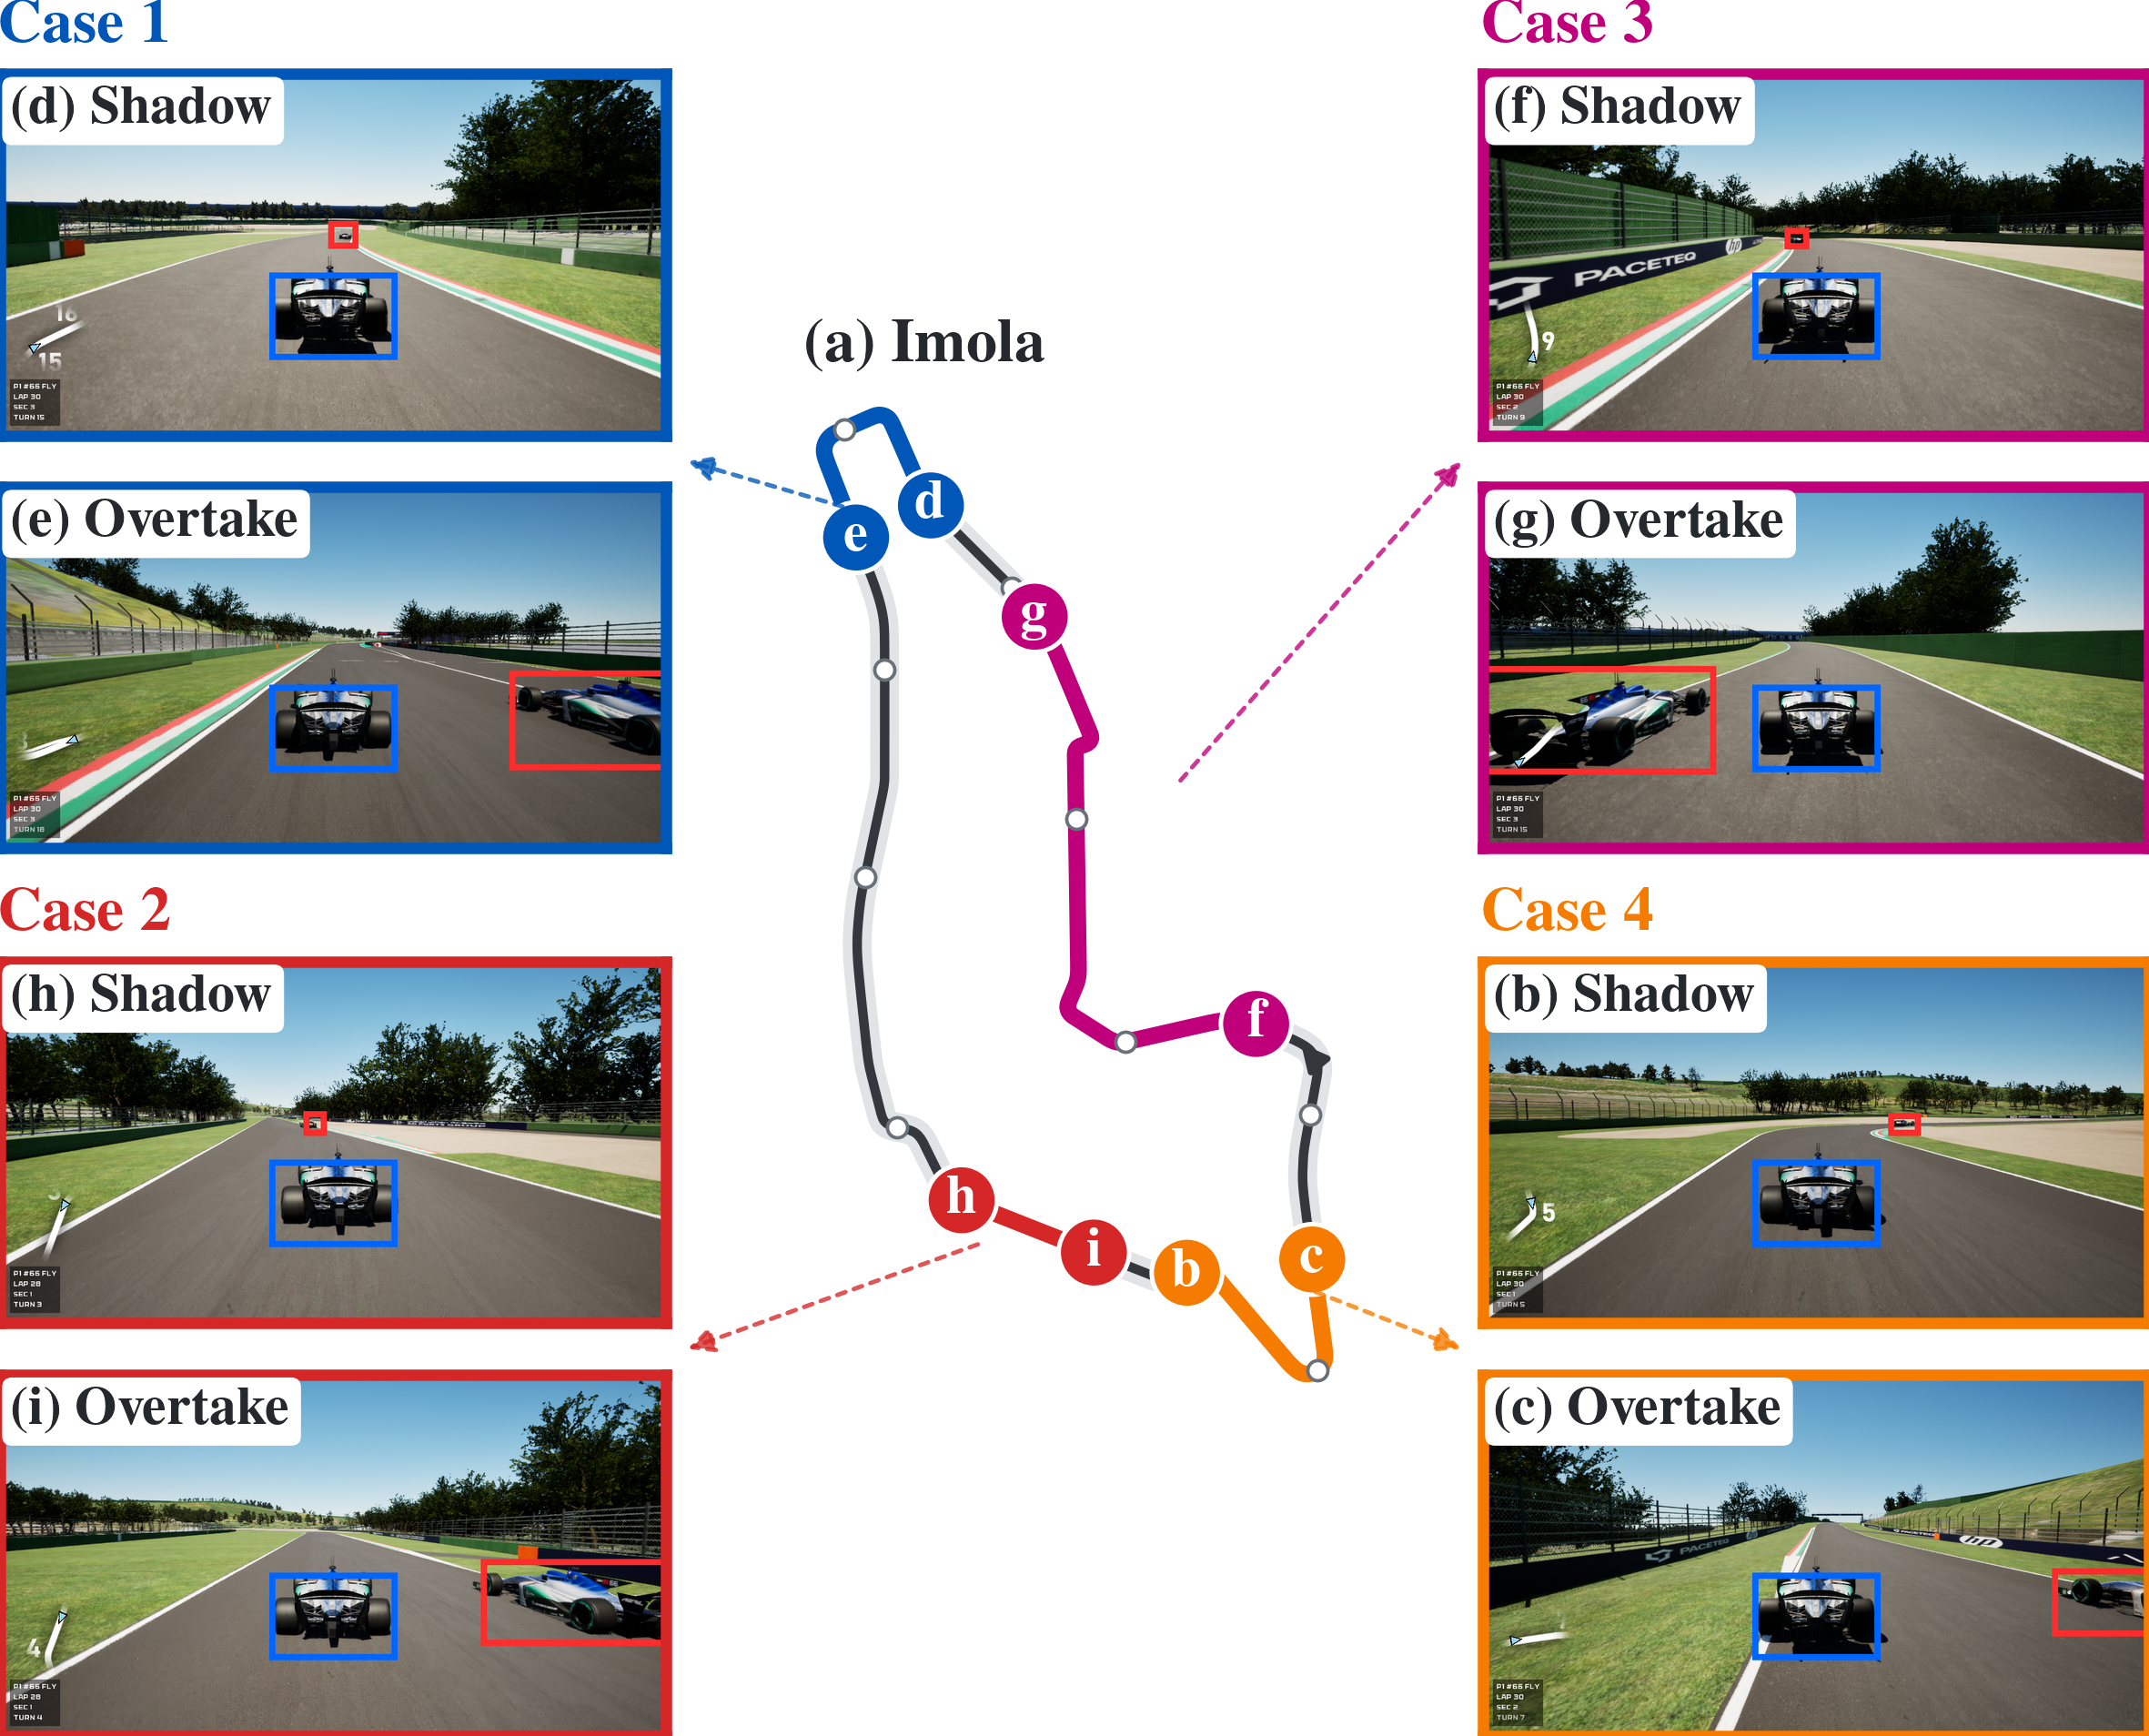
\includegraphics[width=\columnwidth]{track_overview_imola_v006.png}
\caption{Representative overtaking events on the unseen Imola circuit. The
track map localizes four events, with paired \textrm{\textsc{Shadow}} and
\textrm{\textsc{Overtake}} simulator views at each location.}
\label{fig:imola_overview}
\end{figure}

\begin{figure}[!tbp]
\centering
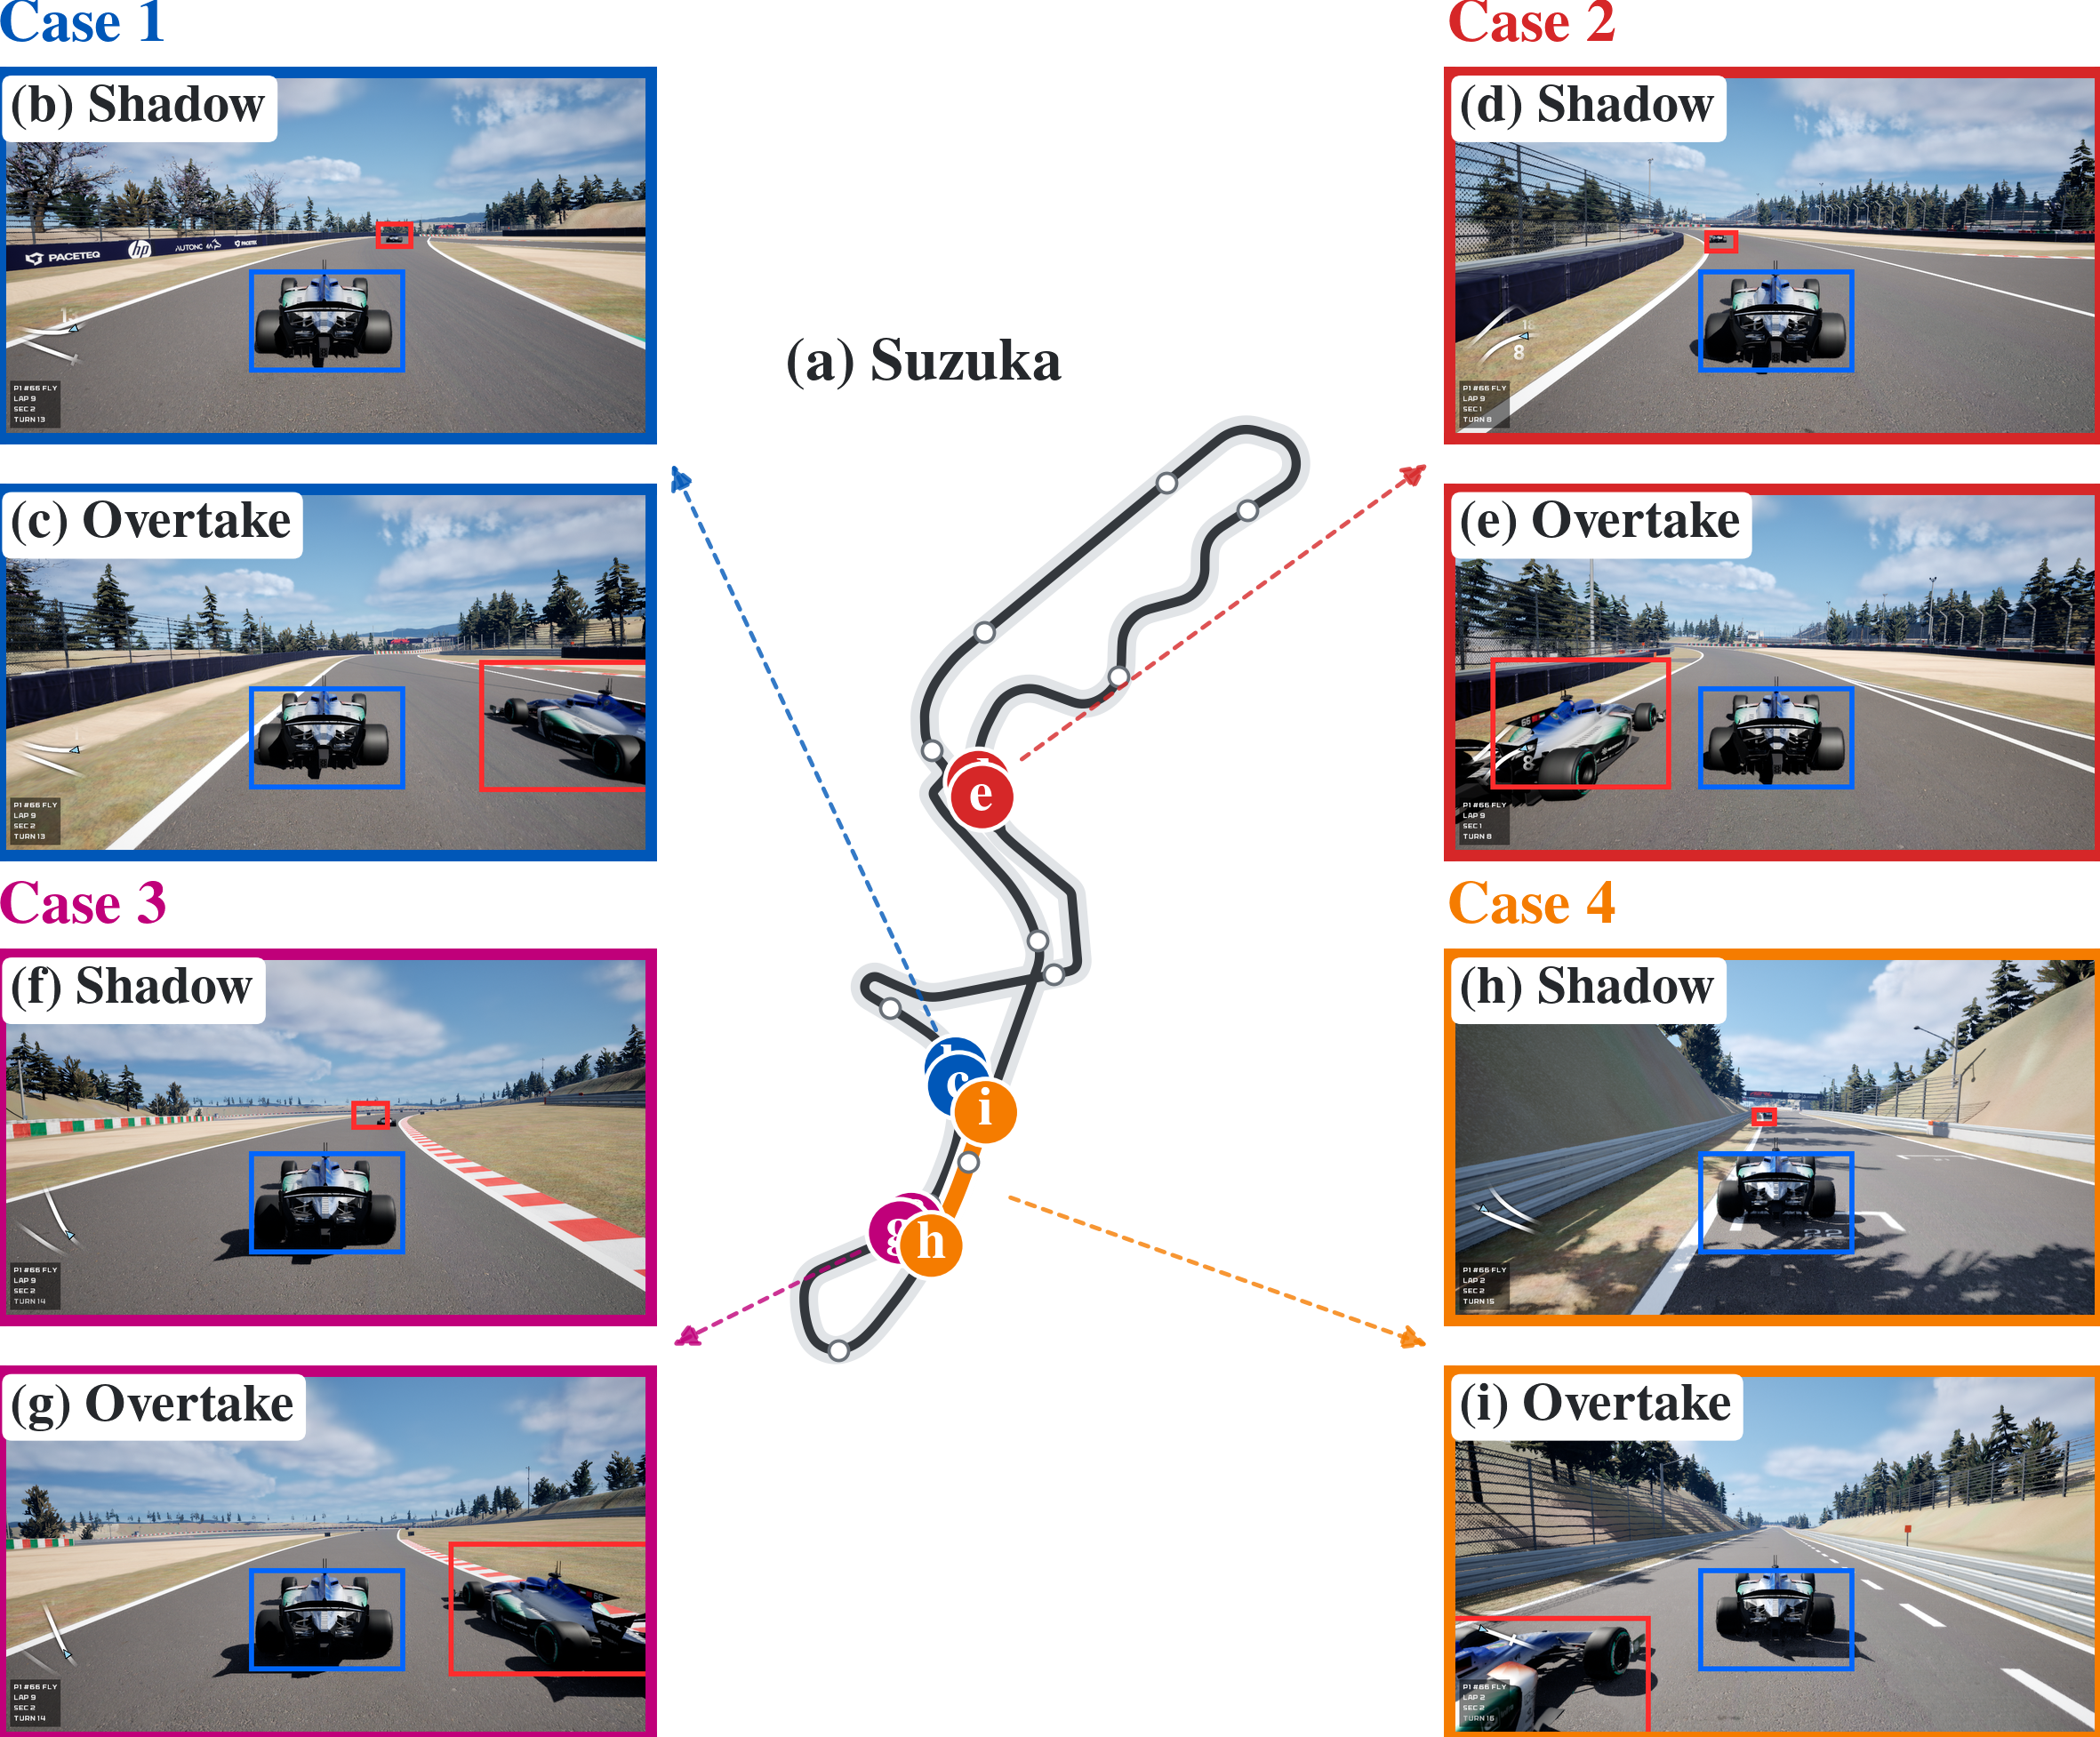
\includegraphics[width=\columnwidth]{track_overview_suzuka_selected_four_v005.png}
\caption{Representative overtaking events on the unseen Suzuka circuit. Four
track locations connect the approach and committed passing phases across
distinct local geometries.}
\label{fig:suzuka_overview}
\end{figure}

\begin{table}[!tbp]
\centering
\footnotesize
\setlength{\tabcolsep}{3.0pt}
\renewcommand{\arraystretch}{1.05}
\caption{Aggregate performance over 1000 Monte Carlo runs on each unseen
circuit.}
\label{tab:unseen_generalization}
\begin{tabular}{@{}lcc@{}}
\toprule
Metric & Imola & Suzuka \\
\midrule
OSR [\%]                      & 91.8 & 88.9 \\
TTO [s]                       & $5.19$ & $4.68$ \\
Minimum gap [m]               & $5.46$ & $5.05$ \\
Mean TTC [s]                  & $8.07$ & $7.45$ \\
Contact rate [\%]             & 0.2 & 0.5 \\
Track-violation rate [\%]     & 0.0 & 0.1 \\
PFR                           & $0.9968$ & $0.9934$ \\
\bottomrule
\end{tabular}

\vspace{1mm}
\begin{minipage}{0.98\columnwidth}
\scriptsize
\emph{Notes:} Continuous entries are Monte Carlo means; TTO is averaged over
successful overtakes. Binary outcomes are reported as percentages.
\end{minipage}
\end{table}

Across the eight illustrated events, the tactical state progresses from
approach to committed passing on both straight and curved sections, while the
corridor remains aligned with the local track geometry. The aggregate outcomes
in Table~\ref{tab:unseen_generalization} quantify this cross-circuit transfer.



% % =====================================================================
% \section{Discussion and limitations}\label{sec:discussion}
% % =====================================================================

% The results identify the persistent tactical feasible region as the principal
% link between interactive reasoning and successful closed-loop overtaking. All
% matched methods share the same executor, yet fixing the corridor produced the
% largest loss in OSR and path feasibility, and removing the FSM produced the
% second largest loss. Response-set supervision further improved passing timing
% and clearance, while TQC provided a complementary gain through distributional
% value learning. This hierarchy supports the central representation: the
% learned corridor creates a spatial passing opportunity, and side commitment
% preserves that opportunity across repeated replanning. It extends the
% update-wise interaction reasoning of dynamic-game solvers
% ~\cite{liniger2019game,wang2021game,fridovich2020ilqgames} and the rapid
% decision capability of learned racing policies
% ~\cite{wurman2022gtsophy,fuchs2021superhuman,song2021overtaking} with an
% explicit space--speed interface for constrained planning.

% Each layer has a distinct role. The response-set teacher evaluates plausible
% opponent reactions; the learned policy publishes the passing side, spatial
% extent, and speed demand; the FSM and carver maintain a connected channel as
% relative geometry changes; and the common executor realizes that channel as
% path--speed motion. The two detailed cases show this sequence during a short
% high-speed pass and a prolonged corner engagement, with tracking and
% acceleration responses compatible with the reference-level tire envelope.
% Target-computer HIL further captures optimization, CAN communication,
% fallback, and actuator-command response throughout this chain.

% The present evaluation covers state-informed, two-vehicle HIL engagements on
% the EAV24 platform, together with geometric transfer tests on Imola and Suzuka.
% The next validation stage will incorporate perception-dependent corridor
% uncertainty, multiple opponents, per-cycle computation statistics, changing
% tire and surface conditions, and matched on-track experiments. These settings
% extend the operating scope of the same persistent feasible-set interface.

% =====================================================================
\section{Conclusion}\label{sec:conclusion}
% =====================================================================
This paper addressed the persistence and executability of opponent-aware
overtaking decisions under repeated replanning. The proposed method represents
the decision as a side-committed, time-varying tactical feasible region. A
robust Stackelberg response-set teacher supervises where and when to form this
region, TQC distils the supervision, and the hysteretic state machine with
deterministic carving maintains it as the encounter evolves. A common
sequential-SOCP and RC-NMPC
executor then converts the published corridor into closed-loop path--speed
motion. On the target RGS-8805GC computer in a dual-CAN EAV24 HIL loop, the
method achieved 94.7\% overtaking success over 1000 Monte Carlo closed-loop
simulations and exceeded four
matched baselines by 31.2--66.2 percentage points. The fixed-corridor and
no-FSM ablations produced the two largest performance losses, directly linking
adaptive feasible-set generation and temporal persistence to successful
execution. These results establish tactical-corridor learning as an effective
interface between interaction reasoning and constrained vehicle planning
within state-informed, two-vehicle autonomous racing.

\appendix
\section{Algorithm and Evaluation Parameters}
\label{app:parameters}
\setcounter{table}{0}

This appendix reports the numerical settings and normalized reward features
needed to reproduce the algorithmic logic.

\begin{table}[!tbp]
\centering
\scriptsize
\setlength{\tabcolsep}{2.0pt}
\renewcommand{\arraystretch}{0.95}
\caption{Principal algorithm and closed-loop evaluation settings.}
\label{tab:setup_params}
\begin{tabular}{@{}p{0.21\linewidth}p{0.43\linewidth}p{0.30\linewidth}@{}}
\toprule
Component & Parameter & Value \\
\midrule
Vehicle geometry & \(m\); \(l_f,l_r\) & \(742\) kg; \(1.75,1.35\) m \\
Tire curves & \(F_{z,0}\); \(C_x,C_y\); \(E_x,E_y\) &
\(2079.72\) N; \(1.6144,1.5998\); \(0,0\) \\
Tire curves & \(\mu_x,\mu_y\); \(s_x,s_y\); \(q_{x,\rm pk},q_{y,\rm pk}\) &
\(2.2345,1.9745\); \(-0.2555,-0.4787\); \(0.1296,0.140\) \\
Tire envelope & construction; online evaluation &
quasi-steady-state map~\eqref{eq:tire_accel_envelope}; speed interpolation \\
Time scales & \(T_{\rm tac}\); \(T_c\); station spacing &
\(0.02\) s; \(0.01\) s; \(2\) m \\
Response-set teacher & Sobol candidates per side; \(\varepsilon_{\rm BR}\);
\(\gamma_g\) & \(64\); \(0.05\); \(0.99\) \\
Action projection & \(\Delta_g\); \(q_{\rm neu}\) & \(0.5\) m; \(0.25\) \\
FSM & \(N_{\rm post}\); stale-reference limit &
\(3\) updates; \(1\) revalidated cycle \\
TQC & critics; \(N_q\); retained \(K\); \(\gamma\) &
\(2\); \(25\); \(46\); \(0.99\) \\
TQC guidance & \(\lambda_p\); \(\lambda_g\); prior metric &
\(1\); \(1\); identity after action normalization \\
Corridor & preview; stations; \(L_{\min}^{\rm corr}\); \(\beta\) &
\(300\) m; \(150\); \(3\) m; \(0.2\) \\
Frenet health & \(\varepsilon_s\); \(\xi_{\max}\); \(\underline v_s\) &
\(0.05\); \(1.30\) rad; \(1\) m s\(^{-1}\) \\
Path health & iterations; \((\varepsilon_{\rm dyn},\varepsilon_{\rm cor})\) &
\(5\); \((10^{-3},10^{-3}\ {\rm m})\) \\
Speed profile & \(H_s\); \(V_{\min},v_{x,\max}\); \(\varepsilon_\rho\) &
\(150\); \(15,90\) m s\(^{-1}\); \(10^{-3}\) \\
RC-NMPC & steps; \(T_c\); \(\delta_{\max}\); \(\dot\delta_{\max}\);
\(\Delta V_{\max}\) &
\(15\); \(0.01\) s; \(0.35\) rad; \(1.0\) rad s\(^{-1}\);
\(0.5\) m s\(^{-1}\) \\
RC-NMPC weights & \(q_{\Delta\delta},q_c,q_\psi\); \(\bm R_\nu\) &
\(2,20,10\); \(\operatorname{diag}(1,0.5)\) \\
\bottomrule
\end{tabular}
\end{table}

\begin{table}[t]
\centering
\scriptsize
\caption{Tactical-policy bounds, reward weights, and training settings.
Symbols follow Eqs.~\eqref{eq:action_vec} and~\eqref{eq:reward_sum}.}
\label{tab:tactical_settings}
\renewcommand{\arraystretch}{0.98}
\begin{tabular}{@{}p{0.29\linewidth}p{0.65\linewidth}@{}}
\toprule
Group & Setting \\
\midrule
Corridor and speed & $L^{\rm cap},R^{\rm cap}\in[1.5,6.0]$ m;
$d_{\rm safe}\in[0.2,0.8]$ m;
$V_{\rm cap}^{\rm req}\in[15,90]$ m s$^{-1}$ \\
Gap thresholds & $g_{\rm chase}\in[18,24]$ m;
$g_{\rm ot}\in[16,24]$ m; $g_{\rm abort}\in[28,45]$ m \\
Bias, recovery, side & $b_{\rm lat}\in[-1.5,1.5]$ m;
$w_{\rm safe}\in[1,5]$ m; $q_{\rm side}\in[-1,1]$ \\
Reward weights & $\bm w=(30,-20,-100,-2,-5,3,-0.1,-0.5,0.5,0.25)$,
ordered as in Eq.~\eqref{eq:reward_sum} \\
Optimization & learning rate $3\times10^{-4}$; replay capacity $10^5$;
batch size $256$; target update $5\times10^{-3}$ \\
Networks & independent actor encoder $51\!\to\!256\!\to\!256$; shared
critic state--action encoder; two quantile heads; training-only robust-value head \\
Projection gradients & piecewise $\Pi_{\mathcal A}$; exact
$\Pi_{\rm tire}$ forward pass with STE for actor/prior updates; detached
Bellman target \\
Software & Python \texttt{3.10.0}; SB3 \texttt{2.8.0}; PyTorch
\texttt{2.4.0+cu124}; Gymnasium \texttt{1.2.3} \\
\bottomrule
\end{tabular}
\end{table}

\begingroup
\scriptsize
\setlength{\jot}{0.5pt}
\begin{equation}
\begin{aligned}
\phi_{\rm ot}&=\mathbb{1}[m_t=\textsc{Overtake},
m_{t+1}=\textsc{Raceline},P_t],\\
\phi_{\rm ovb}&=\phi_{\rm ot}\text{ with roles exchanged},\\
\phi_{\rm col}&=\mathbb{1}[\mathrm{contact}\vee\mathrm{offtrack}
\vee\mathrm{comm\_loss}],\\
\phi_{\rm lat}&=\mathbb{1}[m_t=\textsc{Raceline}]
\operatorname{clip}\!\left(\frac{n_e-n_{\rm rl}}{W_{\rm trk}/2},-1,1\right)^2,\\
\phi_{\rm crush}&=\mathbb{1}[|g_t|<g_{\rm ot}]
\left(\frac{[\rho_{\rm exc}-|\Delta n|]_+}{\rho_{\rm exc}}\right)^2,\\
\phi_{\rm app}&=\mathbb{1}[0<g_t<g_{\rm chase}]
\operatorname{clip}\!\left(\frac{g_{t-1}-g_t}{g_{\rm chase}},0,1\right),\\
\phi_{\rm sm}&=\min\!\left\{1,
\frac{\|\mathsf N_a(\bm a_t^{\rm F})-
\mathsf N_a(\bm a_{t-1}^{\rm F})\|_2^2}{10}\right\},\\
\phi_{\rm gs}&=\min\!\left\{1,\frac{1}{2N_{\rm sta}}
\sum_k\sum_{\pm}\left(\frac{n_{k,t}^{\pm}-n_{k,t-1}^{\pm}}
{W_{{\rm trk},k}}\right)^2\right\},\\
\phi_{\rm sbs}&=\mathbb{1}[|g_t|<g_{\rm ot},
|\Delta n|\ge\rho_{\rm exc}],\\
\phi_{\rm wide}&=\frac{1}{N_{\rm sta}}\sum_k
\operatorname{clip}\!\left(\frac{n_{k,t}^+-n_{k,t}^--L_{\min}^{\rm corr}}
{W_{{\rm trk},k}-L_{\min}^{\rm corr}},0,1\right).
\end{aligned}
\label{eq:reward_features}
\end{equation}
\endgroup



\section*{Acknowledgements}
The authors acknowledge the Abu Dhabi Autonomous Racing League for providing
the EAV24 simulation and vehicle-interface environment.


\renewcommand{\bibfont}{\fontsize{7}{7.8}\selectfont}
\setlength{\bibsep}{-0.1pt}
\begin{thebibliography}{35}

\bibitem{kabzan2020amzracing}
J. Kabzan, M. de la Iglesia Valls, V. J. F. Reijgwart \emph{et al.},
``AMZ Driverless: The full autonomous racing system,''
\emph{Journal of Field Robotics}, vol. 37, no. 7, pp. 1267--1294, 2020.

\bibitem{betz2022survey}
J. Betz, H. Zheng, A. Liniger \emph{et al.},
``Autonomous vehicles on the edge: A survey on autonomous vehicle racing,''
\emph{IEEE Open Journal of Intelligent Transportation Systems}, vol. 3,
pp. 458--488, 2022.

\bibitem{betz2023autonomous}
J. Betz, T. Betz, F. Fent \emph{et al.},
``TUM autonomous motorsport: An autonomous racing software for the Indy
Autonomous Challenge,'' \emph{Journal of Field Robotics}, vol. 40, no. 4,
pp. 783--809, 2023.

\bibitem{jung2023iac}
C. Jung, A. Finazzi, H. Seong \emph{et al.},
``An autonomous system for head-to-head race: Design, implementation and
analysis,'' \emph{IEEE Transactions on Intelligent Transportation Systems},
vol. 24, no. 10, pp. 10470--10486, 2023.

\bibitem{sureshbabu2022autopass}
V. Suresh Babu and M. Behl,
``Threading the needle---Overtaking framework for multi-agent autonomous
racing,'' \emph{SAE International Journal of Connected and Automated
Vehicles}, vol. 5, no. 1, pp. 33--43, 2022,
doi: 10.4271/12-05-01-0004.

\bibitem{kim2023hierarchical}
C. Kim, K. Yi, and J. Park,
``Hierarchical motion planning and control algorithm of autonomous racing
vehicles for overtaking maneuvers,'' in \emph{SAE Technical Paper Series},
2023, Paper 2023-01-0698, doi: 10.4271/2023-01-0698.

\bibitem{ji2023hierarchicalgame}
K. Ji, N. Li, M. Orsag, and K. Han,
``Hierarchical and game-theoretic decision-making for connected and automated
vehicles in overtaking scenarios,'' \emph{Transportation Research Part C:
Emerging Technologies}, vol. 150, art. 104109, 2023,
doi: 10.1016/j.trc.2023.104109.

\bibitem{ji2024competition}
K. Ji, S. Bae, N. Li, and K. Han,
``Competition-aware decision-making approach for mobile robots in racing
scenarios,'' in \emph{Proc. IEEE Intelligent Vehicles Symposium (IV)}, 2024,
pp. 878--884, doi: 10.1109/IV55156.2024.10588596.

\bibitem{swain2023cooperative}
S. K. Swain, J. J. Rath, and K. C. Veluvolu,
``Cooperative game theory based robust shared lateral control for driver
vehicle interactions,'' \emph{Control Engineering Practice}, vol. 141,
art. 105678, 2023, doi: 10.1016/j.conengprac.2023.105678.

\bibitem{lopez2022payoff}
V. Lopez, F. Lewis, M. Liu, Y. Wan, S. Nageshrao, and D. Filev,
``Game-theoretic lane-changing decision making and payoff learning for
autonomous vehicles,'' \emph{IEEE Transactions on Vehicular Technology},
vol. 71, no. 4, pp. 3609--3620, 2022,
doi: 10.1109/TVT.2022.3148972.

\bibitem{liniger2019game}
A. Liniger and J. Lygeros,
``A noncooperative game approach to autonomous racing,''
\emph{IEEE Transactions on Control Systems Technology}, vol. 28, no. 3,
pp. 884--897, 2020.

\bibitem{wang2021game}
M. Wang, Z. Wang, J. Talbot, J. C. Gerdes, and M. Schwager,
``Game-theoretic planning for self-driving cars in multivehicle competitive
scenarios,'' \emph{IEEE Transactions on Robotics}, vol. 37, no. 4,
pp. 1313--1325, 2021.

\bibitem{fridovich2020ilqgames}
D. Fridovich-Keil, E. Ratner, L. Peters, A. D. Dragan, and C. J. Tomlin,
``Efficient iterative linear-quadratic approximations for nonlinear
multi-player general-sum differential games,'' in \emph{Proc. IEEE
International Conference on Robotics and Automation (ICRA)}, 2020,
pp. 1475--1481.

\bibitem{jia2023bayesian}
Y. Jia, M. Bhatt, and N. Mehr,
``RAPID: Autonomous multi-agent racing using constrained potential dynamic
games,'' in \emph{Proc. European Control Conference (ECC)}, 2023, pp. 1--8.

\bibitem{kalaria2025alpha}
D. Kalaria, C. Maheshwari, and S. Sastry,
``$\alpha$-RACER: Real-time algorithm for game-theoretic motion planning and
control in autonomous racing using $\alpha$-potential function,'' in
\emph{Proc. Learning for Dynamics and Control Conference}, PMLR, vol. 283,
pp. 1--18, 2025.

\bibitem{wurman2022gtsophy}
P. R. Wurman, S. Barrett, K. Kawamoto \emph{et al.},
``Outracing champion Gran Turismo drivers with deep reinforcement learning,''
\emph{Nature}, vol. 602, no. 7896, pp. 223--228, 2022.

\bibitem{yuan2022drlgame}
M. Yuan, J. Shan, and K. Mi,
``Deep reinforcement learning based game-theoretic decision-making for
autonomous vehicles,'' \emph{IEEE Robotics and Automation Letters}, vol. 7,
no. 2, pp. 818--825, 2022, doi: 10.1109/LRA.2021.3134249.

\bibitem{fuchs2021superhuman}
F. Fuchs, Y. Song, E. Kaufmann, D. Scaramuzza, and P. D\"urr,
``Super-human performance in Gran Turismo Sport using deep reinforcement
learning,'' \emph{IEEE Robotics and Automation Letters}, vol. 6, no. 3,
pp. 4257--4264, 2021.

\bibitem{evans2023trajectory}
B. D. Evans, H. A. Engelbrecht, and H. W. Jordaan,
``High-speed autonomous racing using trajectory-aided deep reinforcement
learning,'' \emph{IEEE Robotics and Automation Letters}, vol. 8, no. 9,
pp. 5353--5359, 2023, doi: 10.1109/LRA.2023.3295252.

\bibitem{hell2024lidar}
M. Hell, G. Hajgat\'o, \'A. Bog\'ar-N\'emeth \emph{et al.},
``A LiDAR-based approach to autonomous racing with model-free reinforcement
learning,'' in \emph{Proc. IEEE Intelligent Vehicles Symposium (IV)}, 2024,
pp. 258--263, doi: 10.1109/IV55156.2024.10588613.

\bibitem{song2021overtaking}
Y. Song, H. Lin, E. Kaufmann, P. D\"urr, and D. Scaramuzza,
``Autonomous overtaking in Gran Turismo Sport using curriculum reinforcement
learning,'' in \emph{Proc. IEEE International Conference on Robotics and
Automation (ICRA)}, 2021, pp. 9403--9409.

\bibitem{lin2023limit}
H. Lin, Y. Song, and D. Scaramuzza,
``Reaching the limit in autonomous racing: Optimal control versus
reinforcement learning,'' \emph{Science Robotics}, vol. 8, no. 82,
art. eadg1462, 2023.

\bibitem{hu2023dynamicgraph}
X. Hu, Y. Liu, B. Tang, J. Yan, and L. Chen,
``Learning dynamic graph for overtaking strategy in autonomous driving,''
\emph{IEEE Transactions on Intelligent Transportation Systems}, vol. 24,
no. 11, pp. 11921--11933, 2023, doi: 10.1109/TITS.2023.3287223.

\bibitem{baumann2025predictive}
N. Baumann, E. Ghignone, C. Hu, B. Hildisch, T. H\"ammerle,
A. Bettoni, A. Carron, L. Xie, and M. Magno,
``Predictive Spliner: Data-driven overtaking in autonomous racing using
opponent trajectory prediction,'' \emph{IEEE Robotics and Automation
Letters}, vol. 10, no. 2, pp. 1816--1823, 2025,
doi: 10.1109/LRA.2024.3519878.

\bibitem{han2024marl}
S. Han, S. Zhou, J. Wang, L. Pepin, C. Ding, J. Fu, and F. Miao,
``A multi-agent reinforcement learning approach for safe and efficient
behavior planning of connected autonomous vehicles,''
\emph{IEEE Transactions on Intelligent Transportation Systems}, vol. 25,
no. 5, pp. 3654--3670, 2024, doi: 10.1109/TITS.2023.3336670.

\bibitem{liu2023proactive}
Y. Liu, A. Zhou, Y. Wang, and S. Peeta,
``Proactive longitudinal control to preclude disruptive lane changes of
human-driven vehicles in mixed-flow traffic,''
\emph{Control Engineering Practice}, vol. 136, art. 105522, 2023,
doi: 10.1016/j.conengprac.2023.105522.

\bibitem{guo2025rlhf}
H. Guo, R. Khaire, and J. Zhao,
``Reinforcement learning from human feedback with fast--slow updates for
stable driving strategies,'' \emph{Control Engineering Practice}, vol. 165,
art. 106549, 2025, doi: 10.1016/j.conengprac.2025.106549.

\bibitem{muzahid2025merging}
A. J. M. Muzahid, Y. Shi, Z. Wang, A. Zhou, A. Cook, C. R. Wang, and Z. Wang,
``Optimizing on-ramp merging for connected and automated vehicles: A
hierarchical approach using deep reinforcement learning and optimal control,''
\emph{Control Engineering Practice}, vol. 165, art. 106614, 2025,
doi: 10.1016/j.conengprac.2025.106614.

\bibitem{thakkar2024hierarchical}
R. S. Thakkar, A. S. Samyal, D. Fridovich-Keil, Z. Xu, and U. Topcu,
``Hierarchical control for head-to-head autonomous racing,''
\emph{Field Robotics}, vol. 4, no. 1, pp. 46--69, 2024,
doi: 10.55417/FR.2024002.

\bibitem{reiter2023hierarchical}
R. Reiter, J. Hoffmann, J. Boedecker, and M. Diehl,
``A hierarchical approach for strategic motion planning in autonomous
racing,'' in \emph{Proc. European Control Conference (ECC)}, 2023, pp. 1--8,
doi: 10.23919/ECC57647.2023.10178143.

\bibitem{hoffmann2026a2rl}
S. Hoffmann, S. Sagmeister, T. Betz \emph{et al.},
``Head-to-head autonomous racing at the limits of handling in the A2RL
challenge,'' arXiv preprint arXiv:2602.08571, 2026.

\bibitem{kuznetsov2020tqc}
A. Kuznetsov, P. Shvechikov, A. Grishin, and D. Vetrov,
``Controlling overestimation bias with truncated mixture of continuous
distributional quantile critics,'' in \emph{Proc. 37th International
Conference on Machine Learning}, PMLR, vol. 119, pp. 5556--5566, 2020.

\bibitem{yang2026corridor}
C. Yang, H. Liu, Z. Li, X. Zhang, X. Zhao, and B. Wang,
``Hierarchical cooperative planning incorporating MARL guidance and
interactive spatio-temporal corridor constraints,''
\emph{Control Engineering Practice}, vol. 175, art. 107120, 2026,
doi: 10.1016/j.conengprac.2026.107120.

\bibitem{toschi2025modular}
A. Toschi, F. Prignoli, and M. Bertogna,
``Modular decision-making and drivable areas for multi-agent autonomous
racing,'' in \emph{Proc. IEEE/RSJ International Conference on Intelligent
Robots and Systems (IROS)}, 2025, pp. 12435--12441,
doi: 10.1109/IROS60139.2025.11246897.

\bibitem{veneri2020free}
M. Veneri and M. Massaro,
``A free-trajectory quasi-steady-state optimal-control method for minimum
lap-time of race vehicles,''
\emph{Vehicle System Dynamics}, vol. 58, no. 6, pp. 933--954, 2020,
doi: 10.1080/00423114.2019.1608364.

\end{thebibliography}



\end{document}
